% Options for packages loaded elsewhere
\PassOptionsToPackage{unicode}{hyperref}
\PassOptionsToPackage{hyphens}{url}
\PassOptionsToPackage{dvipsnames,svgnames,x11names}{xcolor}
%
\documentclass[
  10pt,
  a4paperpaper,
  DIV=11,
  numbers=noendperiod,
  oneside]{scrreprt}

\usepackage{amsmath,amssymb}
\usepackage{iftex}
\ifPDFTeX
  \usepackage[T1]{fontenc}
  \usepackage[utf8]{inputenc}
  \usepackage{textcomp} % provide euro and other symbols
\else % if luatex or xetex
  \usepackage{unicode-math}
  \defaultfontfeatures{Scale=MatchLowercase}
  \defaultfontfeatures[\rmfamily]{Ligatures=TeX,Scale=1}
\fi
\usepackage{lmodern}
\ifPDFTeX\else  
    % xetex/luatex font selection
\fi
% Use upquote if available, for straight quotes in verbatim environments
\IfFileExists{upquote.sty}{\usepackage{upquote}}{}
\IfFileExists{microtype.sty}{% use microtype if available
  \usepackage[]{microtype}
  \UseMicrotypeSet[protrusion]{basicmath} % disable protrusion for tt fonts
}{}
\makeatletter
\@ifundefined{KOMAClassName}{% if non-KOMA class
  \IfFileExists{parskip.sty}{%
    \usepackage{parskip}
  }{% else
    \setlength{\parindent}{0pt}
    \setlength{\parskip}{6pt plus 2pt minus 1pt}}
}{% if KOMA class
  \KOMAoptions{parskip=half}}
\makeatother
\usepackage{xcolor}
\usepackage[top=25mm,bottom=25mm,left=17.5mm,right=82.5mm,marginparsep=10mm,marginparwidth=55mm]{geometry}
\setlength{\emergencystretch}{3em} % prevent overfull lines
\setcounter{secnumdepth}{5}
% Make \paragraph and \subparagraph free-standing
\makeatletter
\ifx\paragraph\undefined\else
  \let\oldparagraph\paragraph
  \renewcommand{\paragraph}{
    \@ifstar
      \xxxParagraphStar
      \xxxParagraphNoStar
  }
  \newcommand{\xxxParagraphStar}[1]{\oldparagraph*{#1}\mbox{}}
  \newcommand{\xxxParagraphNoStar}[1]{\oldparagraph{#1}\mbox{}}
\fi
\ifx\subparagraph\undefined\else
  \let\oldsubparagraph\subparagraph
  \renewcommand{\subparagraph}{
    \@ifstar
      \xxxSubParagraphStar
      \xxxSubParagraphNoStar
  }
  \newcommand{\xxxSubParagraphStar}[1]{\oldsubparagraph*{#1}\mbox{}}
  \newcommand{\xxxSubParagraphNoStar}[1]{\oldsubparagraph{#1}\mbox{}}
\fi
\makeatother

\usepackage{color}
\usepackage{fancyvrb}
\newcommand{\VerbBar}{|}
\newcommand{\VERB}{\Verb[commandchars=\\\{\}]}
\DefineVerbatimEnvironment{Highlighting}{Verbatim}{commandchars=\\\{\}}
% Add ',fontsize=\small' for more characters per line
\usepackage{framed}
\definecolor{shadecolor}{RGB}{241,243,245}
\newenvironment{Shaded}{\begin{snugshade}}{\end{snugshade}}
\newcommand{\AlertTok}[1]{\textcolor[rgb]{0.68,0.00,0.00}{#1}}
\newcommand{\AnnotationTok}[1]{\textcolor[rgb]{0.37,0.37,0.37}{#1}}
\newcommand{\AttributeTok}[1]{\textcolor[rgb]{0.40,0.45,0.13}{#1}}
\newcommand{\BaseNTok}[1]{\textcolor[rgb]{0.68,0.00,0.00}{#1}}
\newcommand{\BuiltInTok}[1]{\textcolor[rgb]{0.00,0.23,0.31}{#1}}
\newcommand{\CharTok}[1]{\textcolor[rgb]{0.13,0.47,0.30}{#1}}
\newcommand{\CommentTok}[1]{\textcolor[rgb]{0.37,0.37,0.37}{#1}}
\newcommand{\CommentVarTok}[1]{\textcolor[rgb]{0.37,0.37,0.37}{\textit{#1}}}
\newcommand{\ConstantTok}[1]{\textcolor[rgb]{0.56,0.35,0.01}{#1}}
\newcommand{\ControlFlowTok}[1]{\textcolor[rgb]{0.00,0.23,0.31}{\textbf{#1}}}
\newcommand{\DataTypeTok}[1]{\textcolor[rgb]{0.68,0.00,0.00}{#1}}
\newcommand{\DecValTok}[1]{\textcolor[rgb]{0.68,0.00,0.00}{#1}}
\newcommand{\DocumentationTok}[1]{\textcolor[rgb]{0.37,0.37,0.37}{\textit{#1}}}
\newcommand{\ErrorTok}[1]{\textcolor[rgb]{0.68,0.00,0.00}{#1}}
\newcommand{\ExtensionTok}[1]{\textcolor[rgb]{0.00,0.23,0.31}{#1}}
\newcommand{\FloatTok}[1]{\textcolor[rgb]{0.68,0.00,0.00}{#1}}
\newcommand{\FunctionTok}[1]{\textcolor[rgb]{0.28,0.35,0.67}{#1}}
\newcommand{\ImportTok}[1]{\textcolor[rgb]{0.00,0.46,0.62}{#1}}
\newcommand{\InformationTok}[1]{\textcolor[rgb]{0.37,0.37,0.37}{#1}}
\newcommand{\KeywordTok}[1]{\textcolor[rgb]{0.00,0.23,0.31}{\textbf{#1}}}
\newcommand{\NormalTok}[1]{\textcolor[rgb]{0.00,0.23,0.31}{#1}}
\newcommand{\OperatorTok}[1]{\textcolor[rgb]{0.37,0.37,0.37}{#1}}
\newcommand{\OtherTok}[1]{\textcolor[rgb]{0.00,0.23,0.31}{#1}}
\newcommand{\PreprocessorTok}[1]{\textcolor[rgb]{0.68,0.00,0.00}{#1}}
\newcommand{\RegionMarkerTok}[1]{\textcolor[rgb]{0.00,0.23,0.31}{#1}}
\newcommand{\SpecialCharTok}[1]{\textcolor[rgb]{0.37,0.37,0.37}{#1}}
\newcommand{\SpecialStringTok}[1]{\textcolor[rgb]{0.13,0.47,0.30}{#1}}
\newcommand{\StringTok}[1]{\textcolor[rgb]{0.13,0.47,0.30}{#1}}
\newcommand{\VariableTok}[1]{\textcolor[rgb]{0.07,0.07,0.07}{#1}}
\newcommand{\VerbatimStringTok}[1]{\textcolor[rgb]{0.13,0.47,0.30}{#1}}
\newcommand{\WarningTok}[1]{\textcolor[rgb]{0.37,0.37,0.37}{\textit{#1}}}

\providecommand{\tightlist}{%
  \setlength{\itemsep}{0pt}\setlength{\parskip}{0pt}}\usepackage{longtable,booktabs,array}
\usepackage{calc} % for calculating minipage widths
% Correct order of tables after \paragraph or \subparagraph
\usepackage{etoolbox}
\makeatletter
\patchcmd\longtable{\par}{\if@noskipsec\mbox{}\fi\par}{}{}
\makeatother
% Allow footnotes in longtable head/foot
\IfFileExists{footnotehyper.sty}{\usepackage{footnotehyper}}{\usepackage{footnote}}
\makesavenoteenv{longtable}
\usepackage{graphicx}
\makeatletter
\def\maxwidth{\ifdim\Gin@nat@width>\linewidth\linewidth\else\Gin@nat@width\fi}
\def\maxheight{\ifdim\Gin@nat@height>\textheight\textheight\else\Gin@nat@height\fi}
\makeatother
% Scale images if necessary, so that they will not overflow the page
% margins by default, and it is still possible to overwrite the defaults
% using explicit options in \includegraphics[width, height, ...]{}
\setkeys{Gin}{width=\maxwidth,height=\maxheight,keepaspectratio}
% Set default figure placement to htbp
\makeatletter
\def\fps@figure{htbp}
\makeatother

\usepackage{booktabs}
\usepackage[scaled=0.98, sups]{XCharter}
\usepackage[scaled=1.04, varqu, varl]{inconsolata}
\usepackage[type1]{cabin}
\usepackage{algorithm}
\usepackage{algpseudocode}
\usepackage{array}
\usepackage{multirow}
\usepackage{tikz}
\usepackage{framed}
\usepackage{mdframed}
%\usepackage[xcharter, vvarbb, scaled=1.07]{newtxmath}
\usepackage[dvipsnames]{xcolor}
\usepackage{colortbl}
\definecolor{CodeBackground}{HTML}{F0F0F0}
\definecolor{CodeString}{HTML}{008080}
\definecolor{CodeComment}{HTML}{008000}
\definecolor{alertRed}{HTML}{E54B4B}
\usepackage{layout}

\usepackage{fvextra}
\DefineVerbatimEnvironment{Highlighting}{Verbatim}{breaklines,commandchars=\\\{\}}

\newenvironment{cntrlplcy}{}{}

\def\fps@table{htbp}
\usepackage{listings}
\lstset{breaklines=true, columns=flexible, aboveskip=-8pt, belowskip=-10pt, showlines}
\lstdefinelanguage{CMPseudo}{%
  language     = Python,
  morekeywords = {zeros, TRANSITION, TRIGGER, WITH, SCHEDULE, TIME, FOR, IN, WITH, IF, THEN, END, IS, NOT, empty, START, CREATE},
  numbers=left,
  numberstyle=\footnotesize,
  basicstyle = \small \ttfamily,
  keywordstyle = \color{blue},
  stringstyle = \color{CodeString},
  commentstyle=\color{CodeComment},
  showstringspaces = false,
  backgroundcolor=\color{CodeBackground},
}

\lstdefinelanguage{JavaNew}{%
  language     = Java,
  numbers=left,
  numberstyle=\footnotesize,
  backgroundcolor=\color{CodeBackground},
  keywordstyle = \color{blue},
  basicstyle = \small \ttfamily
}

\newlength{\lastcol}

\setcounter{topnumber}{8}
\setcounter{bottomnumber}{8}
\setcounter{totalnumber}{8}

% \pagestyle{myheadings}
% \markright{\rightmark}

\renewcommand*{\partpagestyle}{empty}

\newmdenv[hidealllines=true, innerleftmargin=0cm, innerrightmargin=0cm, innertopmargin=0cm, innerbottommargin=0cm]{codebox}

\newmdenv[nobreak=false, hidealllines=true, backgroundcolor=CodeBackground]{codeout}

\KOMAoption{captions}{tableheading}
\makeatletter
\@ifpackageloaded{float}{}{\usepackage{float}}
\floatstyle{plain}
\@ifundefined{c@chapter}{\newfloat{cntrlplcy}{h}{locntrlplcy}}{\newfloat{cntrlplcy}{h}{locntrlplcy}[chapter]}
\floatname{cntrlplcy}{Control Policy}
\newcommand*\listofcntrlplcys{\listof{cntrlplcy}{List of Control Policys}}
\makeatother
\makeatletter
\@ifpackageloaded{bookmark}{}{\usepackage{bookmark}}
\makeatother
\makeatletter
\@ifpackageloaded{caption}{}{\usepackage{caption}}
\AtBeginDocument{%
\ifdefined\contentsname
  \renewcommand*\contentsname{Table of contents}
\else
  \newcommand\contentsname{Table of contents}
\fi
\ifdefined\listfigurename
  \renewcommand*\listfigurename{List of Figures}
\else
  \newcommand\listfigurename{List of Figures}
\fi
\ifdefined\listtablename
  \renewcommand*\listtablename{List of Tables}
\else
  \newcommand\listtablename{List of Tables}
\fi
\ifdefined\figurename
  \renewcommand*\figurename{Figure}
\else
  \newcommand\figurename{Figure}
\fi
\ifdefined\tablename
  \renewcommand*\tablename{Table}
\else
  \newcommand\tablename{Table}
\fi
}
\@ifpackageloaded{float}{}{\usepackage{float}}
\floatstyle{ruled}
\@ifundefined{c@chapter}{\newfloat{codelisting}{h}{lop}}{\newfloat{codelisting}{h}{lop}[chapter]}
\floatname{codelisting}{Listing}
\newcommand*\listoflistings{\listof{codelisting}{List of Listings}}
\makeatother
\makeatletter
\makeatother
\makeatletter
\@ifpackageloaded{caption}{}{\usepackage{caption}}
\@ifpackageloaded{subcaption}{}{\usepackage{subcaption}}
\makeatother
\makeatletter
\@ifpackageloaded{sidenotes}{}{\usepackage{sidenotes}}
\@ifpackageloaded{marginnote}{}{\usepackage{marginnote}}
\makeatother

\ifLuaTeX
  \usepackage{selnolig}  % disable illegal ligatures
\fi
\usepackage{bookmark}

\IfFileExists{xurl.sty}{\usepackage{xurl}}{} % add URL line breaks if available
\urlstyle{same} % disable monospaced font for URLs
\hypersetup{
  pdftitle={ENGSCI 355 Labs},
  pdfauthor={Thomas Adams},
  colorlinks=true,
  linkcolor={blue},
  filecolor={Maroon},
  citecolor={Blue},
  urlcolor={Blue},
  pdfcreator={LaTeX via pandoc}}


\title{ENGSCI 355 Labs}
\author{Thomas Adams}
\date{2024-08-29}

\begin{document}
\maketitle

\renewcommand*\contentsname{Table of contents}
{
\hypersetup{linkcolor=}
\setcounter{tocdepth}{2}
\tableofcontents
}

\bookmarksetup{startatroot}

\chapter*{Preface}\label{preface}
\addcontentsline{toc}{chapter}{Preface}

\markboth{Preface}{Preface}

These are an online version of the Labs for ENGSCI 355. The topics
covered are: a hands-on simulation of a manufacturing process;
conceptual modelling using HCCM; implementing HCCM models in Jaamsim;
and missing data imputaton.

\part{Practical Lab}

\chapter{Operations System in Practice}\label{sec-hands-on-sim}

The goal of this lab is to give you some hands-on experience with an
operations system, the type of system that we will be focussing on
simulating. Hopefully this will give you some idea of what is needed to
simulate a system in terms of:

\begin{itemize}
\tightlist
\item
  the components of the system and how they interact with each other
  (entities and their behaviour);
\item
  the type and amount of information/data that is needed, both for
  activity durations and control policies;
\item
  the types of experiments that can be performed and how the system can
  be redesigned.
\end{itemize}

\section{Making Paper Cars}\label{making-paper-cars}

The system that we will use as an example is making a car out of paper.
You will each be given a piece of paper with the net of paper car on it
as in Figure~\ref{fig-car_net}.

\begin{marginfigure}

\centering{

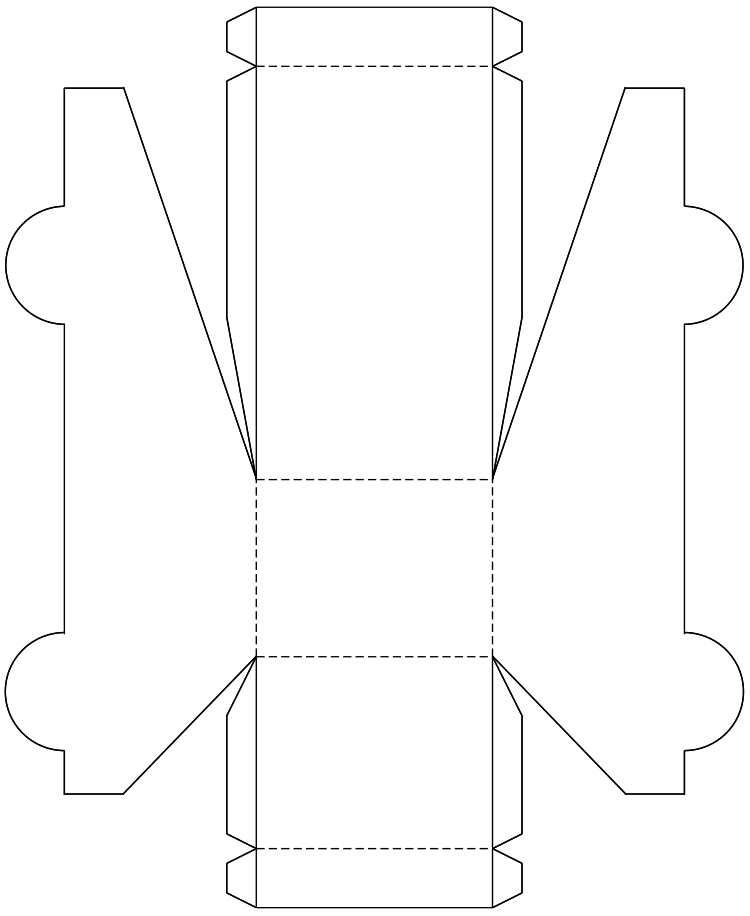
\includegraphics{chapters/hands_on_production/figures/Car_Net_Blank.png}

}

\caption{\label{fig-car_net}The Net Used to Make Paper Cars}

\end{marginfigure}%

You will also get a pair of scissors, some tape, and blank pieces of
paper. To make the car:

\begin{enumerate}
\def\labelenumi{\arabic{enumi}.}
\tightlist
\item
  Trace the net onto a new piece of paper.
\item
  Cut the new net out.
\item
  Fold the paper and tape the edges shut placing the tabs on the inside.
\end{enumerate}

Figure~\ref{fig-car_complete} shows an example of a completed car.

\begin{marginfigure}

\centering{

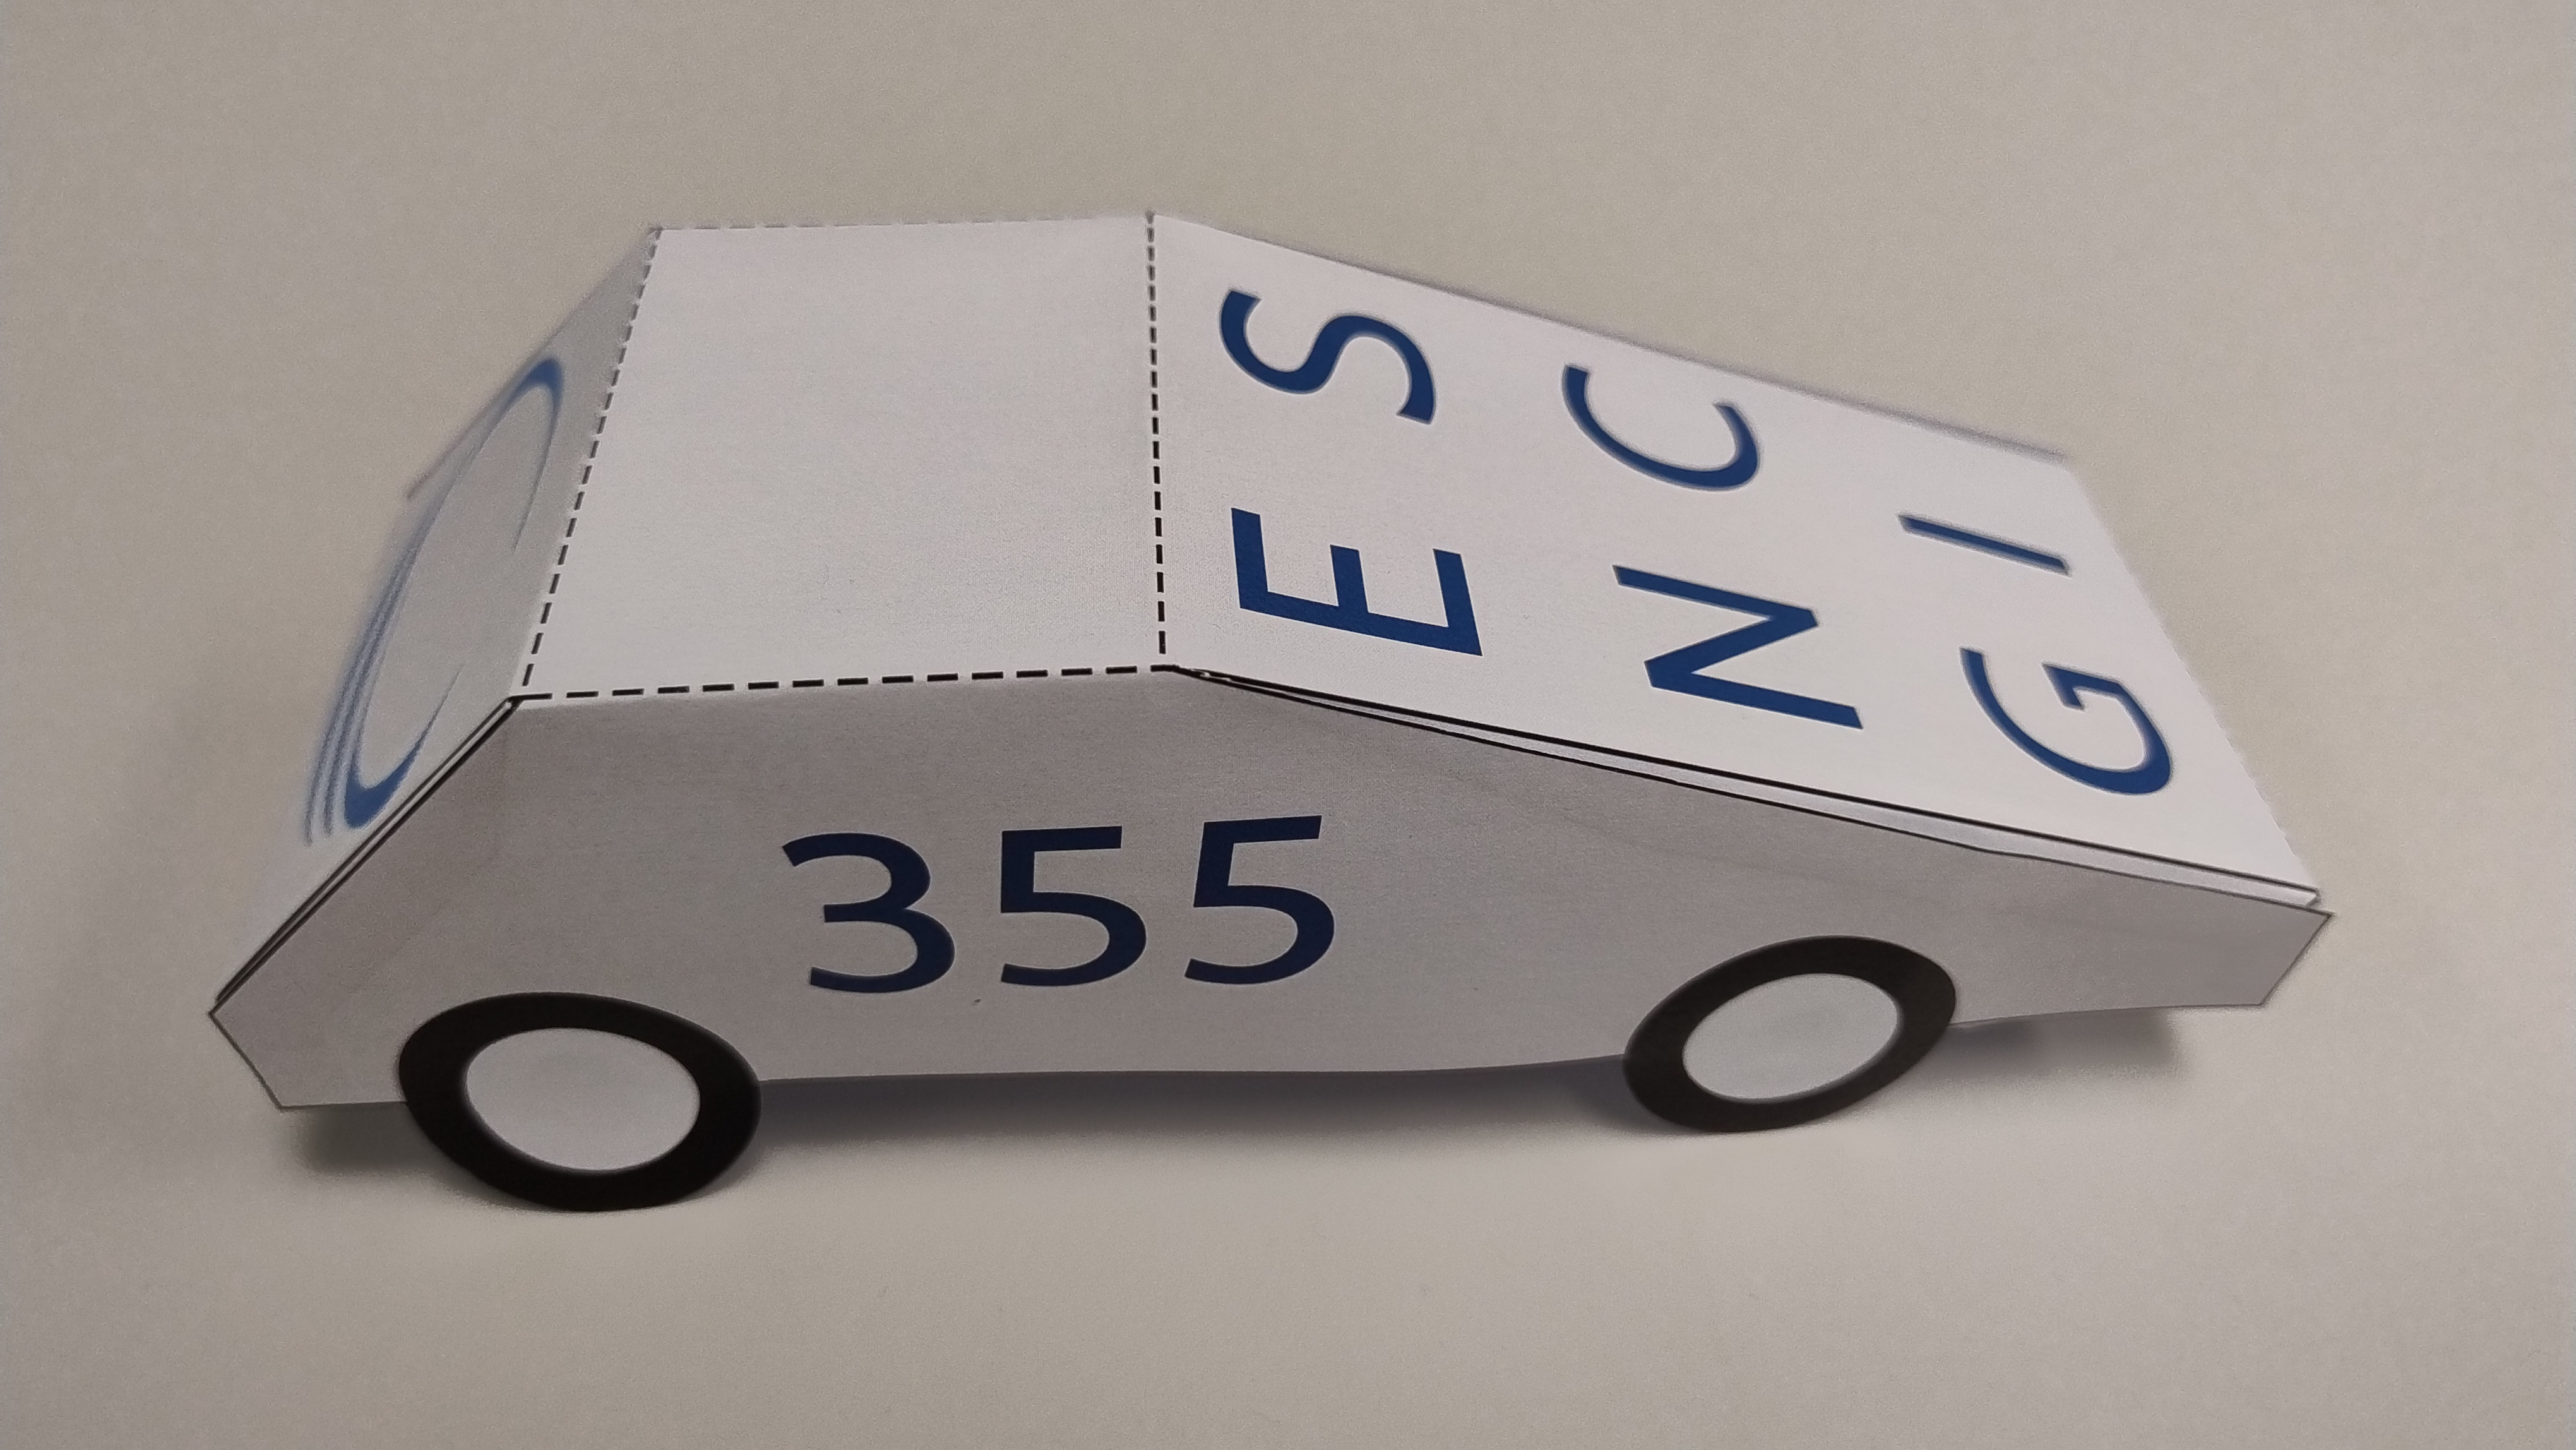
\includegraphics{chapters/hands_on_production/figures/Car_Complete.jpg}

}

\caption{\label{fig-car_complete}A Completed Car}

\end{marginfigure}%

First everyone should make one car by themselves. Once you have, show
one of the instructors to get signed off. Then, discuss with you group
how you can work together to make paper cars. You might want to
experiment with different setups/policies and try making a few cars to
see how long it takes and gather some data.

There will be a competition to see which group can make the most cars in
10 minutes. Before the time starts each group must submit an estimate of
how many cars they believe they will be able to make. The score for each
group will then be comprised of the following elements:

\begin{itemize}
\tightlist
\item
  1 point for each car completed up to and including the estimated
  number.
\item
  0.25 points for each car completed above the estimated number.
\item
  -0.75 points for each car not completed in the estimated number.
\end{itemize}

Additionally, the following rules must be followed:

\begin{enumerate}
\def\labelenumi{\arabic{enumi}.}
\tightlist
\item
  Each car must be traced and cut individually.
\item
  Cars must be the same shape as the original template, including tabs.
\item
  You can have as many stencils as you like.
\item
  All final cars must have started as a blank, unfolded piece of paper.
\item
  You may not have any pre-cut tape or nets.
\item
  All cars must have been made only by members of your group.
\item
  All cars must be folded and taped neatly to count. The lecturer has
  final say on whether a car meets the required neatness.
\end{enumerate}

\section{Reflections}\label{reflections}

Now that you have attempted to make as many cars as you can you may wish
to reflect on the process by asking yourself the following questions:

\begin{itemize}
\tightlist
\item
  Did your group have any traced/cut out cars left at the end?
\item
  What was the bottleneck/slowest part of the system?
\item
  Did you collect any data/do any experiments? If so, did they help?
  Would you do more/different ones now?
\item
  What would you do differently next time?
\end{itemize}

The process that we considered was relatively simple. Cinsider how would
your group's strategy change if any of the following additional
conditions were added:

\begin{itemize}
\tightlist
\item
  Blank pieces of paper for you to trace onto only become available one
  at a time every two minutes;
\item
  You have to make different styles of cars on demand;
\item
  There is a limit to how many traced nets/cut pieces of tape you can
  have at any point (buffer limit);
\item
  Each time a pair of scissors is stopped being used there is a cooldown
  time of 1 minute.
\end{itemize}

\part{Conceptual Modelling Labs}

\chapter{HCCM Framework}\label{hccm-framework}

This chapter describes the Hierarchical Control Conceptual Modelling
(HCCM) framework which is used to build a conceptual model, aligned with
the HCCM standard from lectures, that represents the practical activity,
i.e., making paper cars, from Chapter~\ref{sec-hands-on-sim}.

Working in the same groups as for the practical activity and using this
chapter as guidance, over the next two labs you will work through the
phases for HCCM modelling shown in Figure~\ref{fig-cm_phases} and
complete templates for those steps. In the next lab you will complete
phases 1, 2, 3, and start phase 4. The remainder of phase 4 will be
completed in the lab after that. Chapter~\ref{sec-hands-on-sim} provides
a partially completed conceptual model of the car making system that you
can use as a starting point.

\begin{figure*}[htbp]

\centering{

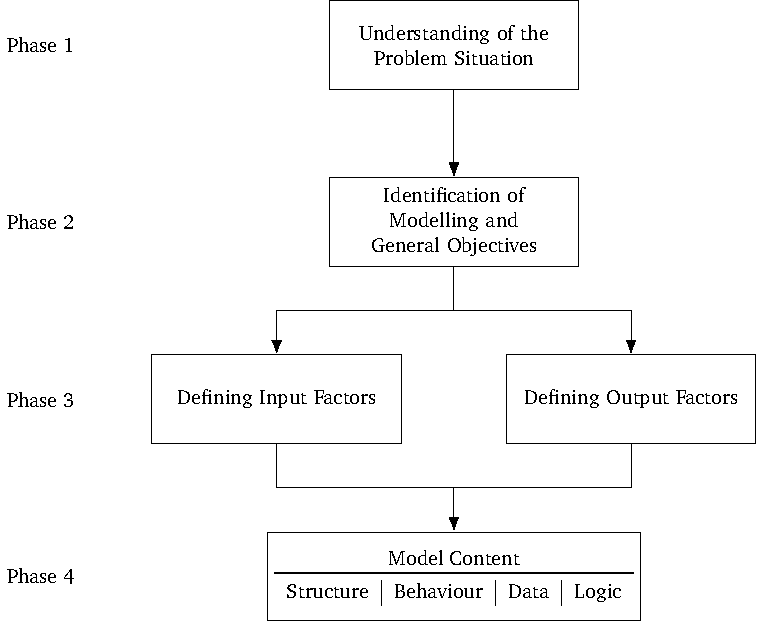
\includegraphics[width=129mm,height=\textheight]{chapters/hccm_framework/figures/cm_phases.pdf}

}

\caption{\label{fig-cm_phases}Conceptual Modelling Phases}

\end{figure*}%

\section{Understanding of the Problem
Situation}\label{understanding-of-the-problem-situation}

In Phase 1, in order to understand the problem situation, you need to
summarise what is happening in a concise way. There is no strict rule
for the best way to do this. One good approach is listening to the
problem ``holder'', i.e., person/people who have the problem such as a
client, then reflecting what you have heard in a couple of paragraphs
with lists of key details and questions. You can then work through one
or more iterations of feedback and refinement to get a final, agreed
upon problem description.

\section{Identification of Modelling and General
Objectives}\label{identification-of-modelling-and-general-objectives}

For Phase 2, as described in lectures, there are two types of objectives
to consider when developing a simulation:

\begin{quote}
``The second step deals with the determination of the objectives.
According to Robinson {[}26{]} they drive all aspects of the modeling
process and are a subset of an organization's aims. Further, objectives
can be classified into modeling and general objectives, where the latter
are concerned with the flexibility, run-speed, visual-display and
model/component reuse.''
\end{quote}

For the modelling objective you may like to think about what you trying
to discover using simulation, and what level of performance you are
trying to achieve in which areas/metrics.

\section{Defining Output Responses}\label{defining-output-responses}

Phase 3 includes defining both the output responses and input factors.
You can do these in either order, but it can often be useful to define
the output responses first, as it may help you think about what inputs
will influence the outputs.

Output responses are things that can be measured and compared to
understand how a system has behaved/performed. They are the metrics used
to compare different simulation scenarios. The output responses should
let you know whether the modelling objectives have been achieved and why
or how. You may also want to consider how this will be reported (tables,
graphs, etc.).

\section{Defining Input Factors}\label{defining-input-factors}

Input factors are things that can be changed and may modify how a system
behaves/performs. They are often defined to create multiple different
scenarios to compare via simulation. They are also what you can change
to try and achieve the modelling objectives.

\section{Model Content}\label{model-content}

In Phase 4 the model content is defined. There is no strict order in
which you need to complete the four components (structre, behaviour,
data, and logic). A possible approach, that we will take in this lab, is
to:

\begin{enumerate}
\def\labelenumi{\arabic{enumi}.}
\tightlist
\item
  Identify the entities;
\item
  Draw the behavioural paths;
\item
  Define the data;
\item
  Define the structure (including the entities again);
\item
  Define the logic.
\end{enumerate}

Using this approach you may still find yourself deciding to add/remove
parts that you have already defined. This is a normal part of the
conceptual modelling process, and you need to go back to the part of the
process you want to change -- for example adding and entity or activity
-- and then update the rest of the CM.

For the model content definition of our conceptual model we will follow
the new HCCM standard. This standard is presented in an academic article
(currently under review) that is available on Canvas under
\texttt{Files > Lectures > Conceptual Modelling} in the file
\href{https://canvas.auckland.ac.nz/courses/113292/files/folder/Lectures/Conceptual\%20Modelling?preview=12376819}{hccm-standard.pdf}

\subsection{Identifying Entities}\label{identifying-entities}

Before formally defining entities it is often useful to identify
entities in the system and whether they are active, i.e., have behaviour
like a doctor or patient, or passive, i.e., are part of the system that
should be modelled but that don't have explicit behaviour like a waiting
room with a given capacity, but that doesn't actually have defined
actions.

The goal is to identify everything that is involved in a meaningful way
in all of the activities that are important to the system. Thinking
about the inputs and outputs can also be useful. Clearly the entities
must be influenced in some way by the inputs, and they must themselves
influence the outputs. You may also consider that an activity does not
have a significant influence on the performance of the system, and
decide to exclude it -- and therefore any entities that are involved
only in that activity. Likewise the participation of a particular entity
in an activity might be deemed inconsequential and therefore excluded.
Although it is possible to revisit and add/remove entities later, at
this stage you want to consider the whole system carefully, as it is
easier to include/exclude an entity now than to change it later.

\subsection{Drawing Behavioural Paths}\label{drawing-behavioural-paths}

Once preliminary identification of entities has been done, behavioural
paths for each of the active entities should be drawn. These are
essentially flowcharts with a special structure. Circles represent
events, usually used when entities are arriving and leaving. Rectangles
represent activities, including when entities have to wait for another
activity. Red squares at the top left of an activity (or sometimes an
event) let us know that some logic is triggered when the activity
starts. This generally occurs at the start of ``wait'' activities and is
used to check whether the conditions that mean the entity can stop
waiting and move on to the next activity are met.

What we are trying to do when drawing the behavioural paths is identify
the activities and events that the entities participate in, the possible
orders that these can occur in, and any points where some control logic
needs to be used.

Both when identifying the entities and drawing the behavioural paths it
is important to keep track of any assumptions and simplifications that
you make.

\subsection{Define the Data}\label{define-the-data}

The data for the conceptual model includes both variables, and data
modules. Variables can change their value throughout the simulation and
are generally used to store some information temporarily before it is
required later in the simulation. Data modules contain the information
that is needed to perform the simulation and can be collected
beforehand. Data mocules can also represent the input/experimental
factors -- the things that may change between different simulation
scenarios. For each data module the following information should be
given:

\begin{enumerate}
\def\labelenumi{\arabic{enumi}.}
\tightlist
\item
  The name of the data module;
\item
  The source of the data, where the information was obtained;
\item
  The way the data is modelled, is it represented by a constant, a
  distribution, etc.
\item
  Whether the output is deterministic or stochastic;
\item
  The inputs that the module requires;
\item
  The quantity that the module outputs.
\end{enumerate}

When presenting a conceptual model is useful to put the data first, as
it is often referenced throughout the rest of the conceptual model.

\subsection{Define the Structure}\label{define-the-structure}

To define the structure we start with formally defining the entities by
listing them along with any attributes that they have. Some common
attributes, such as ID number and the activity that the entity is
currently participating in, are often omitted to avoid repitition.
Attributes are usually included either to assist with the system
behaviour -- for example record whether a patient has had a test -- or
to capture the perfomance of the system -- how long something has waited
for.

Next we define the transitions. Each arrow on a behavioural diagram
corresponds to a transition. We can collate these in a table describing:
the entity that is performing the transition, and the events that the
entity transitions from and to. You can simply number them starting from
1, or adopt a convention of using the entity's initial as a prefix.

Once the transitions have been defined we can define the activities and
events. Usually these are presented in two tables, one for the
activities and one for the events. For each event (either standalone or
as part of an activity) the table should include:

\begin{enumerate}
\def\labelenumi{\arabic{enumi}.}
\tightlist
\item
  The participant(s);
\item
  The type -- either scheduled or controlled;
\item
  The state changes that occur when the event happens.
\end{enumerate}

The main things that occur in state changes are:

\begin{itemize}
\tightlist
\item
  Schedule an end event -- usually in the start event of an activity
  with a scheduled end event;
\item
  Starting another activity/event -- this usually happens in a scheduled
  end event where an entity is transitioning to another scheduled event;
\item
  Trigger some logic -- often in the start event of an activity with a
  controlled end event.
\end{itemize}

The simulation start event, and arrive events are often more complicated
and involve scheduling the initial events and creating entities.

\subsection{Define the Logic}\label{define-the-logic}

The final part of the conceptual model content is the logic. Each
trigger that you drew in a behvioural path (the red squares) should
correspond first to a trigger statement in the state changes of an
event, and a piece of logic defined here. These pieces of logic are used
to determine how the system behaves -- what activity an entity should do
next. It is common to have logic control the behaviour when one entity
needs to wait for another, as when the first entity arrives it needs to
check whether the other is free to perform an activity with it. The
logic is usually presented as pseudocode, alongside the entity that
triggers the logic.

\section{Assumptions and
Simplifications}\label{assumptions-and-simplifications}

Throughout the four phases of the HCCM framework you should document the
assumptions and simplifications that you make. Assumptions are related
to uncertainties about the system being modelled, and are used to fill
in gaps in the information that is required for the simulation.
Simplifications are changes that are made to the model to make it easier
to defined or implement.

\chapter{Inputs, Outputs, and
Behaviour}\label{inputs-outputs-and-behaviour}

In this lab you will complete the first three Phases of the HCCM
framework, and part of the fourth, with your group.

\section{Understanding of the Problem
Situation}\label{understanding-of-the-problem-situation-1}

In the box below write a problem description for making paper cars,
think about what you are trying to solve/discover by simulating this
activity. You may want to look at Chapter~\ref{sec-hands-on-sim} again
to remind yourself about the process.

\begin{figure*}

\begin{mdframed}[innerbottommargin=3cm]

~

~

~

~

~

~

~

~

\end{mdframed}

\end{figure*}%

\section{Modelling Objectives}\label{modelling-objectives}

In the box below write the modelling objectives for making paper cars,
i.e., what are you trying to discover using simulation?

\begin{figure*}

\begin{mdframed}[innerbottommargin=3cm]

~

~

~

~

~

~

~

~

\end{mdframed}

\end{figure*}%

\newpage{}

\section{General Objectives}\label{general-objectives}

In the box below write the general objectives for making paper cars,
i.e., what are some of the general properties you'd like your simulation
to have?

\begin{figure*}

\begin{mdframed}[innerbottommargin=4.5cm]

~

~

~

~

~

~

~

~

~

~

\end{mdframed}

\end{figure*}%

\section{Defining Output Responses}\label{defining-output-responses-1}

In the box below write the output responses for making paper cars, i.e.,
what are you going to measure to determine the performance of the
system?

\begin{figure*}

\begin{mdframed}[innerbottommargin=4.5cm]

~

~

~

~

~

~

~

~

~

~

\end{mdframed}

\end{figure*}%

\newpage{}

\section{Defining Input Factors}\label{defining-input-factors-1}

In the box below write the input factors for making paper cars, i.e.,
what are you going to change to achieve the modelling objectives?

\begin{figure*}

\begin{mdframed}[innerbottommargin=4.5cm]

~

~

~

~

~

~

~

~

~

~

\end{mdframed}

\end{figure*}%

\section{Identifying Entities}\label{identifying-entities-1}

In the box below list the entities for making paper cars.

\begin{figure*}

\begin{mdframed}[innerbottommargin=4.5cm]

~

~

~

~

~

~

~

~

~

~

\end{mdframed}

\end{figure*}%

\newpage{}

\section{Drawing Behavioural Paths}\label{drawing-behavioural-paths-1}

The activity diagrams for the pencil \& template, and scissors are given
below in Figures~\ref{fig-pencil_act}, and~\ref{fig-scissors_act}.

\begin{figure}[htbp]

\centering{

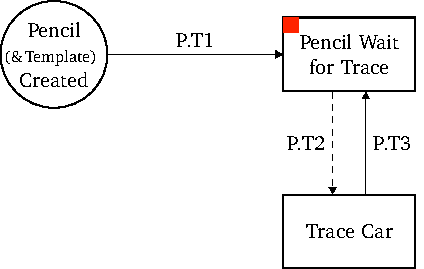
\includegraphics[width=72mm,height=\textheight]{chapters/cm_io_behaviour/figures/pencil-activity.pdf}

}

\caption{\label{fig-pencil_act}Pencil Activity Diagram}

\end{figure}%

\begin{figure}[htbp]

\centering{

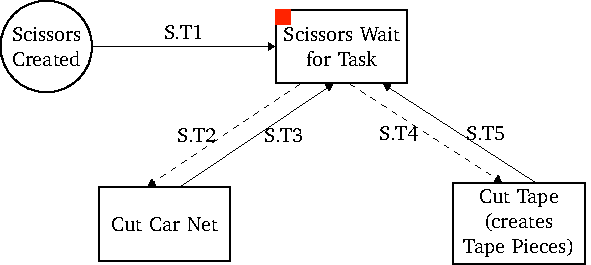
\includegraphics[width=100mm,height=\textheight]{chapters/cm_io_behaviour/figures/scissors-activity.pdf}

}

\caption{\label{fig-scissors_act}Scissors Activity Diagram}

\end{figure}%

\newpage{}

In the boxes below draw the activity diagrams for the remaining
entities.

\begin{figure*}

\begin{mdframed}[innerbottommargin=8cm]
~

~

~

~

~

~

~

~

~

~

~

~

~

~

~

~

~

~

~

~

~

~

~

~

~

~

\end{mdframed}

\end{figure*}%

~

\begin{figure*}

\begin{mdframed}[innerbottommargin=5cm]
~

~

~

~

~

~

~

~

~

~

~

~

~

\end{mdframed}

\end{figure*}%

~

\begin{figure*}

\begin{mdframed}[innerbottommargin=5cm]
~

~

~

~

~

~

~

~

~

~

~

~

~

\end{mdframed}

\end{figure*}%

~

\begin{figure*}

\begin{mdframed}[innerbottommargin=7cm]
~

~

~

~

~

~

~

~

~

~

~

~

~

~

~

~

\end{mdframed}

\end{figure*}%

\chapter{Data, Structure, and Logic}\label{data-structure-and-logic}

In this lab you will complete the remainder of the fourth phase of the
HCCM framework, with your group.

\section{Define the Data}\label{define-the-data-1}

Firstly, you need to give detailed definitions of the data modules. You
may not have collected data during car making, but complete the
following table that describes the kind of data you would need to
collect to simulate car making. Also add a comment on how the entry for
CutTapeDuration would change if no person-by-person data was available,
but an Exponential distribution that estimated the time it takes for a
person to cut tape was available.

\begin{table*}

\caption{\label{tbl-data_pc}List of Data Modules}

\centering{

\begin{tabular}{llllll}
  \toprule
    Name & Source & Model & Type & Input & Output \\ \midrule
    NumPencils & System info & Constant & Deterministic & - & The number of pencils available \\
    NumScissors & System info & Constant & Deterministic & - & The number of scissors available \\
    NumTape & System info & Constant & Deterministic & - & The number of rolls of tape available \\
    Num & System info & Constant & Deterministic & - &  \\
     &  &  &  & &  \\
    TraceCar & Experimental data & Lookup & Deterministic & Person & Time to trace car \\
    CutNet & Experimental data & Lookup & Deterministic & Person & Time to cut the net out \\
    &  &  &  & &  \\
    &  &  &  & &  \\
    &  &  &  & &  \\
    &  &  &  & &  \\
    &  &  &  & &  \\
    &  &  &  & &  \\
    CutTape & Experimental data & Lookup & Deterministic & Person & Time to cut a piece of tape \\ \bottomrule
  \end{tabular}

}

\end{table*}%

\section{Define the Structure}\label{define-the-structure-1}

The first part of the structure to define is the entities.
Table~\ref{tbl-entities_pc} lists the entities again, but adds
attributes that the entities will need to capture the performance of the
system, e.g., waiting time until the cube was cut. It is assumed that
all entities have the three attributes: ID, CurrentActivity, and
CurrentStart. These are omitted in the table to prevent repetition.

\begin{table}

\caption{\label{tbl-entities_pc}List of Entities}

\centering{

\begin{tabular}{ll}
\toprule
Entity  & Attributes        \\ \midrule
Paper   & WaitForTrace[0.0]    \\
        & WaitForCutShape[0.0] \\
        & WaitForFold[0.0]     \\
        & WaitForTapeCube[0.0] \\
        &                      \\
Pencil  & WaitForTrace[0.0]    \\
        &                      \\
Scissors& WaitForTask[0.0]     \\
        &                      \\
Tape    & WaitForCut[0.0]      \\
        &                      \\
TapePieces  & WaitForTape[0.0] \\
        & ArrivalTime[0.0]     \\
        & LeavingTime[0.0]     \\
Person  & WaitForTask[0.0]     \\ \bottomrule
\end{tabular}

}

\end{table}%

The next part of the structure is the transitions, which describe how
entities move between activities and events.
Table~\ref{tbl-transitions_pc} lists the transitions for making paper
cars. These transitions are prefixed by entity of the behavioural
pathway they come from. Complete the transitions for the Scissors
pathway.

\begin{longtable}{p{2.4cm}>{\raggedright\arraybackslash}p{1.2cm}>{\raggedright\arraybackslash}p{5.9cm}>{\raggedright\arraybackslash}p{5.9cm}}

\caption{\label{tbl-transitions_pc}List of Transitions}

\tabularnewline

\toprule
Participant & Name & From Event & To Event       \\ \midrule
\endhead
Paper & PAP.1 & Paper Created & Paper Wait for Trace.Start \\
      & PAP.2 & Paper Wait for Trace.End & Trace Car.Start \\
      & PAP.3 & Trace Car.End & Paper Wait for Cut Net.Start \\
      & PAP.4 & Paper Wait for Cut Net.End & Cut Car Net.Start \\
      & PAP.5 & Cut Car Net.End & Car Wait for Fold.Start \\
      & PAP.6 & Car Wait for Fold.End & Fold Car.Start \\
      & PAP.7 & Fold Car.End & Car Wait for Tape.Start \\
      & PAP.8 & Car Wait for Tape.End & Tape Car.Start \\
      & PAP.9 & Tape Car.End & Car Finished \\
      &      &              &              \\
Pencil & PEN.1 & Pencil/Template Created & Pencil Wait for Trace.Start \\
       & PEN.2 & Pencil Wait for Trace.End & Trace Car.Start \\
       & PEN.3 & Trace Car.End & Pencil Wait for Trace.Start \\
       &      &              &              \\
Scissors & S.1 & Scissors Created             &              \\
       & S.2   &              &              \\
       & S.3   &              &              \\
       & S.4   &              &              \\
       & S.5   &              &              \\
       &      &              &              \\
Tape   & T.1 & Tape Created & Tape Wait for Cut.Start \\
       & T.2 & Tape Wait for Cut.End & Cut Tape.Start \\
       & T.3 & Cut Tape.End & Tape Wait for Cut.Start \\
       &      &              &              \\
Tape Piece & TP.1 & Tape Pieces Created & Tape Pieces Wait for Tape.Start \\
           & TP.2 & Tape Pieces Wait for Tape.End & Tape Car.Start \\
           & TP.3 & Tape Car.End & Tape Pieces Leave \\
     &      &              &              \\
Person & PER.1 & Person Created & Person Wait for Task.Start \\
       & PER.2 & Person Wait for Task.End & Trace Car.Start \\
       & PER.3 & Trace Car.End & Person Wait for Task.Start \\
       & PER.4 & Person Wait for Task.End & Cut Car Net.Start \\
       & PER.5 & Cut Car Net.End & Person Wait for Task.Start \\
       & PER.6 & Person Wait for Task.End & Fold Car.Start \\
       & PER.7 & Fold Car.End & Person Wait for Task.Start \\
       & PER.8 & Person Wait for Task.End & Cut Tape.Start \\
       & PER.9 & Cut Tape.End & Person Wait for Task.Start \\
       & PER.10 & Person Wait for Task.End & Tape Car.Start \\
       & PER.11 & Tape Car.End & Person Wait for Task.Start \\\bottomrule

\end{longtable}

Table~\ref{tbl-activities_pc} lists the activities from the behavioural
pathway diagrams along with the state changes for the start and end
event of each activity. Complete the activities for:

\begin{itemize}
\tightlist
\item
  Car Wait for Tape Car
\item
  Tape Car
\item
  Person Wait for Task (\emph{Hint} look at Scissors Wait for Task)
\end{itemize}

\begin{longtable}{@{}>{\raggedright\arraybackslash}p{1.8cm}>{\raggedright\arraybackslash}p{2.1cm}>{\raggedright\arraybackslash}p{0.9cm}>{\raggedright\arraybackslash}p{2.2cm}>{\raggedright\arraybackslash}p{8.75cm}@{}}

\caption{\label{tbl-activities_pc}Activities}

\tabularnewline

  \toprule
  Activity                                   & Participants                                             & Event & Type       & State Change \\ \midrule
  \endhead
  Paper Wait for Trace      & Paper (P)                            & Start & Scheduled  & 
\begin{lstlisting}[language=CMPseudo]
(Default, omitted hereafter) P.CurrentActivity = "this activity"
(Default, omitted hereafter) P.CurrentStart = TIME
TRIGGER OnStartPaperWaitForTrace WITH C
\end{lstlisting}             \\
                                             &                                                          & End   & Controlled &
  \begin{lstlisting}[language=CMPseudo]
P.WaitForTrace = TIME - P.CurrentStart
# TRANSITION PAP.2 in logic
  \end{lstlisting}              \\ \midrule
  Trace Car                 & Paper (P), Person (H), Pencil (N)       & Start & Controlled &  
\begin{lstlisting}[language=CMPseudo]
SCHEDULE END at TIME + TraceCube(H)
\end{lstlisting}              \\
                                             &                                                          & End   & Scheduled  & 
\begin{lstlisting}[language=CMPseudo]
START Paper Wait for Cut Net WITH P # TRANSITION PAP.3
START Person Wait for Task WITH H # TRANSITION PER.3
START Pencil Wait for Trace WITH N # TRANSITION PEN.3
\end{lstlisting}              \\ \midrule
  Paper Wait for Cut Net    &                                & Start &   & 
\begin{lstlisting}[language=CMPseudo]
TRIGGER OnStartPaperWaitForCutNet WITH P
\end{lstlisting}              \\
  &                                                          & End   &  & 
\begin{lstlisting}[language=CMPseudo]
P.WaitForCutNet = TIME - P.CurrentStart
# TRANSITION PAP.4 in logic
\end{lstlisting}             \\ \midrule
  Cut Car Net               & Paper (P), Person (H), Scissors (S)     & Start & Controlled  & 
\begin{lstlisting}[language=CMPseudo]
SCHEDULE END at TIME + CutNet(H)
\end{lstlisting}             \\
  &                                                          & End   & Scheduled &
\begin{lstlisting}[language=CMPseudo]
START Car Wait for Fold WITH P # TRANSITION PAP.5
START Person Wait for Task WITH H # TRANSITION PER.5
START Scissors Wait for Task WITH S # TRANSITION S.3
\end{lstlisting}              \\ \midrule
  Car Wait for Fold         & Paper (P)                              & Start & Scheduled  & 
\begin{lstlisting}[language=CMPseudo]
TRIGGER OnStartCarWaitForFold WITH P
\end{lstlisting}             \\
  &                                                          & End   & Controlled & 
\begin{lstlisting}[language=CMPseudo]
P.WaitForFold = TIME - P.CurrentStart
# TRANSITION PAP.6 in logic
\end{lstlisting}             \\ \midrule
  Fold Car                  & Paper (P), Person (H)                  & Start & Controlled  & 
\begin{lstlisting}[language=CMPseudo]
SCHEDULE END at TIME + FoldCar(H)
\end{lstlisting}             \\
  &                                                          & End   & Scheduled & 
\begin{lstlisting}[language=CMPseudo]
START Car Wait for Tape Car WITH P # TRANSITION PAP.7
START Person Wait for Task WITH H # TRANSITION PER.7
\end{lstlisting}             \\ \midrule
  \textcolor{Red}{Car Wait for Tape Car}     &                                & Start &   & 
\begin{lstlisting}[language=CMPseudo]
 
\end{lstlisting}             \\
  &                                                          & End   &  & 
\begin{lstlisting}[language=CMPseudo]
 
 
\end{lstlisting}             \\ \midrule
  \textcolor{Red}{Tape Car}                  &  & Start &   & 
\begin{lstlisting}[language=CMPseudo]
 
\end{lstlisting}             \\
  &                                                          & End   &  &
\begin{lstlisting}[language=CMPseudo]
 
 
 
\end{lstlisting}              \\ \midrule
  Pencil Wait for Trace    & Pencil (N)                             & Start & Scheduled  & 
\begin{lstlisting}[language=CMPseudo]
TRIGGER OnStartPencilWaitForTrace WITH N
\end{lstlisting}             \\
  &                                                          & End   & Controlled & 
\begin{lstlisting}[language=CMPseudo]
N.WaitForTrace = N.WaitForTrace + TIME - N.CurrentStart
# TRANSITION N.2 in logic
\end{lstlisting}             \\ \midrule
  Scissors Wait for Task    & Scissors (S)                            & Start & Scheduled  & 
\begin{lstlisting}[language=CMPseudo]
TRIGGER OnStartScissorsWaitForTask WITH S
\end{lstlisting}             \\
  &                                                          & End   & Controlled & 
\begin{lstlisting}[language=CMPseudo]
S.WaitForTask = S.WaitForTask + TIME - S.CurrentStart
# TRANSITION S.2 or S.4 in logic
\end{lstlisting}             \\ \midrule
  Cut Tape                  & Tape (T), Person (H), Scissors (S)      & Start & Controlled  & 
\begin{lstlisting}[language=CMPseudo]
SCHEDULE END at TIME + CutTape(H)
\end{lstlisting}             \\
  &                                                          & End   & Scheduled & 
\begin{lstlisting}[language=CMPseudo]
START Person Wait for Task WITH H # TRANSITION PER.9
START Scissors Wait for Task WITH S # TRANSITION S.5
START Tape Wait for Cut WITH T # TRANSITION T.3
CREATE Tape Pieces TP
START Tape Pieces Created WITH TP
\end{lstlisting}             \\ \midrule
  Tape Wait for Cut         & Tape (T)                                & Start & Scheduled  & 
\begin{lstlisting}[language=CMPseudo]
TRIGGER OnStartTapeWaitForCut WITH T
\end{lstlisting}             \\
  &                                                          & End   & Controlled & 
\begin{lstlisting}[language=CMPseudo]
T.WaitForCut = T.WaitForCut + TIME - T.CurrentStart
# TRANSITION T.2 in logic
\end{lstlisting}             \\ \midrule
  Tape Pieces Wait for Tape & Tape Pieces (TP)                       & Start & Scheduled  & 
\begin{lstlisting}[language=CMPseudo]
TRIGGER OnStartTapePiecesWaitForTape WITH TP
\end{lstlisting}             \\
  &                                                          & End   & Controlled & 
\begin{lstlisting}[language=CMPseudo]
TP.WaitForTape = TP.WaitForTape + TIME - TP.CurrentStart
# TRANSITION TP.2 in logic
\end{lstlisting}             \\ \midrule
\textcolor{Red}{Person Wait for Task}      &     & Start &   & 
\begin{lstlisting}[language=CMPseudo]
 
\end{lstlisting}             \\
  &                                                          & End   &  & 
\begin{lstlisting}[language=CMPseudo]
 
 
\end{lstlisting}             \\ \bottomrule
  

\end{longtable}

Table~\ref{tbl-events_pc} lists the events to start and finish the
simulation along with the events from the behavioural pathway diagrams
along with the state changes for each event. Complete the activities
for:

\begin{itemize}
\tightlist
\item
  Tape Pieces Created
\item
  Person Created
\end{itemize}

\begin{longtable}{@{}>{\raggedright\arraybackslash}p{1.5cm}>{\raggedright\arraybackslash}p{2.1cm}>{\raggedright\arraybackslash}p{2.2cm}>{\raggedright\arraybackslash}p{10cm}@{}}

\caption{\label{tbl-events_pc}Events}

\tabularnewline

  \toprule
  Event          & Participants & Type       & State Change \\ \midrule
  \endhead
  Simulation Start & None  & Scheduled  & 
  \begin{lstlisting}[language=CMPseudo]
FOR NumPaper DO
  CREATE Paper P
  START Paper Created WITH P
END FOR
FOR NumPencils DO
  CREATE Pencil N
  START Pencil/Template Created WITH N
END FOR
FOR NumScissors DO
  CREATE Scissors S
  START Scissors Created WITH S
END FOR
FOR NumTape DO
  CREATE Tape T
  START Tape Created WITH T
END FOR
FOR NumPeople DO
  CREATE Person H
  START Person Created WITH H
END FOR
  \end{lstlisting}
  \\ \midrule
  Paper Created & Paper (P)  & Scheduled  & 
  \begin{lstlisting}[language=CMPseudo]
START Paper Wait for Trace WITH P # TRANSITION PAP.1
  \end{lstlisting}
  \\ \midrule
  Car Finished & Paper (P)  & Scheduled  & 
  \begin{lstlisting}[language=CMPseudo]
Calculate statistics for P
  \end{lstlisting}
  \\ \midrule
  Pencil/ Template Created & Pencil (N)  & Scheduled  & 
  \begin{lstlisting}[language=CMPseudo]
START Pencil Wait for Trace WITH N # TRANSITION PEN.1
  \end{lstlisting}
  \\ \midrule
  Scissors Created & Scissors (S)  & Scheduled  & 
  \begin{lstlisting}[language=CMPseudo]
START Scissors Wait for Task WITH S # TRANSITION S.1
  \end{lstlisting}
  \\ \midrule
  Tape Created & Tape (T)  & Scheduled  & 
  \begin{lstlisting}[language=CMPseudo]
START Tape Wait for Cut WITH T # TRANSITION T.1
  \end{lstlisting}
  \\ \midrule
  \textcolor{Red}{Tape Pieces Created} &   &  & 
  \begin{lstlisting}[language=CMPseudo]
  
  \end{lstlisting}
  \\ \midrule
Tape Pieces Leave & Tape Pieces (TP)  & Scheduled  & 
  \begin{lstlisting}[language=CMPseudo]
Calculate statistics for TP
  \end{lstlisting}
  \\ \midrule
  \textcolor{Red}{Person Created} &  &   & 
  \begin{lstlisting}[language=CMPseudo]
 
  \end{lstlisting}
  \\ \midrule
  Simulation Finish & None  & Scheduled  & 
  \begin{lstlisting}[language=CMPseudo]
Calculate statistics as required for Pencils, Scissors, Tape, Person entities
  \end{lstlisting}
  \\ \bottomrule
  

\end{longtable}

\section{Define the Logic}\label{define-the-logic-1}

The last part of the structure to define is the logic. You need to
define the logic for each of the triggers (the red squares in the
behavioural paths, and TRIGGER statements in the state changes). Tables
XXX show the logic for some of the triggers. Complete the logic for: -
On Tape Wait for Cut.Start - On Cube Wait for Fold.Start - the last
condition of On Person Wait for Task.Start

\begin{longtable}{@{}>{\raggedright\arraybackslash}p{0.25cm}>{\raggedright\arraybackslash}p{13cm}@{}}

\caption{\label{tbl-start_wait_check_in}OnStartPencilWaitForTrace}

\tabularnewline

  \toprule
   & Triggered by: Pencil N\\ \midrule 
  &
\begin{lstlisting}[language=CMPseudo]
IF (any Paper P with P.CurrentActivity = Paper Wait for Trace) AND
   (any Person H with H.CurrentActivity = Person Wait for Task) THEN
    SELECT valid Paper P
    SELECT valid Person H
    START Trace Car WITH P, H, N
END IF
\end{lstlisting}
  \\ \bottomrule
  

\end{longtable}

\part{Jaamsim Labs}

\chapter{Setting Up VSCode and Java}\label{setting-up-vscode-and-java}

In this lab you will walk through the set up of running a Java program
in VSCode. You will need to be able to do this to implement HCCMs in
Jaamsim.

If you do not already have VSCode installed on your machine, download
and install the version appropriate for your operating system from
\href{https://code.visualstudio.com/Download}{here}.

If you are using your own laptop, it is best to install a recent version
of the Java JDK (unless you are confident you already have a recent
version). We recommend Amazon Corretto 21. You can download it from
\href{https://docs.aws.amazon.com/corretto/latest/corretto-21-ug/downloads-list.html}{here},
and then install it.

To see short videos of the steps described below please visit this
\href{https://auckland.au.panopto.com/Panopto/Pages/Sessions/List.aspx?folderID=e07b3856-7cf5-4024-8c93-b21f016633ea}{site}.

Open VSCode, then on the left-hand side click on the Extensions tab.
Search for the `Extension Pack for Java' and install it.

Create a new folder called \textbf{ENGSCI355}, if you are using a lab
computer create this folder on your H drive. If you aren't, then create
it within Documents or wherever you usually keep University related
work. Inside the \textbf{ENGSCI355} folder create another folder called
\textbf{Java\_Example}. Then in VSCode open this folder by going File
-\textgreater{} Open Folder, then navigating to the
\textbf{Java\_Example} folder.

Once you have opened the folder in VSCode, create a new file in it
called \textbf{Hello.java}. Once you have that file (or any .java file)
open VSCode should detect that you are editing a java file and, if there
isn't one already, create a Java Project in the same folder. You should
see that the `Java Projects' section has been enabled in the bottom left
of the screen.

We now want to make sure that this Java Project is using the correct
Java JDK. Hover your mouse over the `Java Projects' title and then click
on the three dots that appear on the right hand side (with the tooltip
`More Actions'), and select `Configure Java Runtime'. Use the drop-down
menu that appears to select the Amazon Corretto 21 JDK. If it is not on
the list, select `Find a local JDK' and browse to the location that you
installed the Amazon Corretto JDK.

Now go back to the Hello.java file and add the following code:

\begin{Shaded}
\begin{Highlighting}[numbers=left,,]
\KeywordTok{public} \KeywordTok{class}\NormalTok{ Hello }\OperatorTok{\{}
  \KeywordTok{public} \DataTypeTok{static} \DataTypeTok{void} \FunctionTok{main}\OperatorTok{(}\BuiltInTok{String}\OperatorTok{[]}\NormalTok{ args}\OperatorTok{)} \OperatorTok{\{}
    \BuiltInTok{System}\OperatorTok{.}\FunctionTok{out}\OperatorTok{.}\FunctionTok{println}\OperatorTok{(}\StringTok{"Hello!"}\OperatorTok{);}
  \OperatorTok{\}}
\OperatorTok{\}}
\end{Highlighting}
\end{Shaded}

To run the program either click on the `Run' button just above the line
that declares the main function, or click on the run button in the top
right corner of the screen. You should see a line with `Hello!' printed
by itself.

You have now create and run a Java program! If you run into any issues,
there are more detailed instructions available
\href{https://code.visualstudio.com/docs/java/java-tutorial}{here}.

\chapter{Setting Up JaamSim and HCCM}\label{setting-up-jaamsim-and-hccm}

In this lab you will walk through the set up of how to run JaamSim from
source in a VSCode project and how to include the HCCM library in
JaamSim.

\section{Prerequisites}\label{prerequisites}

These instructions were prepared using:

\begin{enumerate}
\def\labelenumi{\arabic{enumi}.}
\tightlist
\item
  Git -- 2.47.0.2;
\item
  GitHub Desktop -- 3.4.8 (x64);
\item
  Java -- Amazon Corretto JRE 21;
\item
  VSCode -- 1.95.1.
\end{enumerate}

They should work with more recent versions of the software too. All of
this software is standard on Engineering lab machines. Amazon Corretto
JRE 21 is available on the University of Auckland's Software Centre.

To see short videos of the steps described below please visit this
\href{https://auckland.au.panopto.com/Panopto/Pages/Sessions/List.aspx?folderID=59000722-14f5-4215-8948-b22501731784}{site}.

\section{Create the Project Folder
Structure}\label{create-the-project-folder-structure}

Create a new folder on your H drive called ENGSCI355. Then create three
folders within this one, called \textbf{sim}, \textbf{labs}, and
\textbf{workspace}. The \textbf{sim} folder will contain the java code
for the simulation software Jaamsim, including custom code that you
write, and is the focus of these instructions. The \textbf{labs} folder
will contain subfolders for each lab with the simulation files for each.
Create a folder for HCCM logic functions within the \textbf{sim} folder.
We will use \textbf{sim\_custom} in these instructions.

\section{Clone HCCM into the project
folder}\label{clone-hccm-into-the-project-folder}

Open GitHub Desktop and go to File \(\rightarrow\) Clone repository,
then select the URL tab and enter

\begin{quote}
https://github.com/mosu001/hccm
\end{quote}

as the URL. Choose the Local path to be the \textbf{sim} folder that you
just created.

into an hccm folder within the \textbf{sim} folder. This will create an
\textbf{hccm} folder within the \textbf{sim} folder that contains the
HCCM and Jaamsim code.

Note, if you use git from the command line, e.g., Git Bash, you need to
add the recurse submodules option

\texttt{git\ clone\ -\/-recurse-submodules\ https://github.com/mosu001/hccm}

\section{Create files to load HCCM and customised
components}\label{create-files-to-load-hccm-and-customised-components}

From \textbf{hccm\_custom} copy both \textbf{autoload.cfg} and
\textbf{hccm.inc} into the \textbf{sim\_custom} folder. Then open
\textbf{autoload.cfg} with VSCode and edit it so that the content
matches that in Figure~\ref{fig-inc}.

\begin{figure}[htbp]

\centering{

\begin{verbatim}
Include units.inc
Include sim.inc
Include units-imperial.inc
Include units-knots.inc
Include displayModels.inc
Include graphics.inc
Include probabilityDistributions.inc
Include basicObjects.inc
Include resourceObjects.inc
Include examples.inc
Include processFlow.inc
Include calculationObjects.inc
Include fluidObjects.inc
Include submodels.inc
Include hccm.inc
Include sim_custom.inc
\end{verbatim}

}

\caption{\label{fig-inc}Customised autoload.cfg File}

\end{figure}%

Then rename \textbf{hccm.inc} to \textbf{sim\_custom.inc}, open it in
VSCode, and delete all the contents so it is blank. Don't forget to save
both \textbf{autoload.cfg} and \textbf{sim\_custom.inc}.

\section{Create a VSCode Java
Project}\label{create-a-vscode-java-project}

In VSCode use File \(\rightarrow\) Open Folder to open the \textbf{sim}
folder. In the File Explorer open some folder so that you can see a
.java file and open it, for example:
hccm\textbackslash custom\textbackslash hccm\textbackslash Constants.java.
VSCode should then recognise that you have opened a Java file and the
Java Projects pane should appear.

\section{Configure Source Folders}\label{configure-source-folders}

Now we need to tell VSCode where the source code of the project is. To
do this we click on the three dots at the right of the `Java Projects'
title and select `Configure Classpath'. A new menu should come up that
allows you to add and remove sources. If anything other than
\textbf{hccm\textbackslash custom} is already there remove it by
clicking on the x on the far right hand side, then `Apply Settings'. Add
new sources by clicking on `Add Source Root'. First add
\textbf{sim\textbackslash hccm\textbackslash jaamsim\textbackslash src\textbackslash main\textbackslash java},
then click `Apply Settings'. Then add both
\textbf{sim\textbackslash hccm\textbackslash jaamsim\textbackslash src\textbackslash main\textbackslash resources}
and \textbf{sim\textbackslash sim\_custom}, remembering to apply the
settings after each one.

You can check to make sure that you have the correct sources configured
by opening the \textbf{settings.json} file in the \textbf{.vscode}
folder. Under ``java.project.sourcePaths'' there should be the following
four entries:

\begin{itemize}
\tightlist
\item
  hccm\textbackslash\textbackslash custom
\item
  hccm\textbackslash\textbackslash jaamsim\textbackslash\textbackslash src\textbackslash\textbackslash main\textbackslash\textbackslash java
\item
  hccm\textbackslash\textbackslash jaamsim\textbackslash\textbackslash src\textbackslash\textbackslash main\textbackslash\textbackslash resources
\item
  sim\_custom
\end{itemize}

\section{Configure JDK}\label{configure-jdk}

We need to make sure that VSCode is using the version of Java that we
want it to. To do this we click on the three dots at the right of the
`Java Projects' title and select `Configure Java Runtime'. A drop-down
menu for JDK should come up. Make sure that JavaSE-21 is selected and
then click `Apply Settings'.

\section{Configure Libraries}\label{configure-libraries}

JaamSim also needs the gluegen and jogl libraries to run. These are
packaged with JaamSim as .jar files (a compiled Java program). They can
be added by opening the project settings by clicking on the three dots
at the right of the `Java Projects' title and selecting either
`Configure Java Runtime' or `Configure Classpath'. Then select the
`Libraries' tab on the right. Click on `Add Library', then navigate to
hccm\textbackslash jaamsim\textbackslash jar, select all of the files,
and click `Select Jar File'. Then click `Apply Settings'.

\section{Integrate with JaamSim}\label{integrate-with-jaamsim}

To integrate HCCM and any custom logic with JaamSim you need to copy
your \textbf{autoload.cfg} and \textbf{sim\_custom.inc} files (from
\textbf{sim\_custom}) to
sim\textbackslash hccm\textbackslash jaamsim\textbackslash src\textbackslash main\textbackslash resources\textbackslash resources\textbackslash inputs
and replace the autoload.cfg file that is currently there. You also need
to copy the file \textbf{hccm.inc} in hccm\textbackslash custom to the
same location. To check that they have been copied correctly you can
look in the `Java Projects' section on the left-hand side. Under
hccm\textbackslash jaamsim\textbackslash src\textbackslash main\textbackslash resources\textbackslash resources\textbackslash inputs
you should see both \textbf{hccm.inc} and \textbf{sim\_custom.inc}. If
you don't, try using the menu accessed by clicking the three dots and
selecting `Refresh'.

\section{Run Custom JaamSim}\label{run-custom-jaamsim}

You should now be able to run JaamSim with the HCCM objects enabled.
Start by clicking on the `Run and Debug' menu on the left-hand side,
then click on `create a launch.json file', and select `Java' from the
list of debuggers that comes up in the middle of the screen. By doing
this VSCode analyses the source code to determine which java files you
might like to run and creates run configurations for each of them. In
the file that is created you should see an entry with the name
`GUIFrame', this is the class that we need to run to start JaamSim. To
make the view work correctly when JaamSim is running you need to add
another parameter called ``vmArgs'' with the following entries enclosed
in double quotes and separated by spaces on a single line:

\begin{itemize}
\tightlist
\item
  -\/-add-exports java.base/java.lang=ALL-UNNAMED
\item
  -\/-add-exports java.desktop/sun.awt=ALL-UNNAMED
\item
  -\/-add-exports java.desktop/sun.java2d=ALL-UNNAMED
\end{itemize}

The final entry in the .launch file should look like this:

\begin{figure*}

\begin{Shaded}
\begin{Highlighting}[numbers=left,,]
\StringTok{"type"}\OperatorTok{:} \StringTok{"java"}\OperatorTok{,}
\StringTok{"name"}\OperatorTok{:} \StringTok{"GUIFrame"}\OperatorTok{,}
\StringTok{"request"}\OperatorTok{:} \StringTok{"launch"}\OperatorTok{,}
\StringTok{"mainClass"}\OperatorTok{:} \StringTok{"com.jaamsim.ui.GUIFrame"}\OperatorTok{,}
\StringTok{"projectName"}\OperatorTok{:} \StringTok{"sim\_d11998cc"}\OperatorTok{,}
\StringTok{"vmArgs"}\OperatorTok{:} \StringTok{"{-}{-}add{-}exports java.base/java.lang=ALL{-}UNNAMED {-}{-}add{-}exports java.desktop/sun.awt=ALL{-}UNNAMED {-}{-}add{-}exports java.desktop/sun.java2d=ALL{-}UNNAMED"}
\end{Highlighting}
\end{Shaded}

\end{figure*}%

Then, in the top left-hand corner next to the green play button click on
the drop-down menu and select `GUIFrame'. Then click the green play
button to run JaamSim. The launch screen should appear but you might
also have to click on the JaamSim icon in the Taskbar at the bottom of
the screen to open JaamSim. You should see the `HCCM' palette at the
bottom of the `Model Builder' window, and be able to drag and drop
objects into the View.

\section{Running an HCCM Model}\label{running-an-hccm-model}

Now that we have JaamSim running with the HCCM objects we can try
running an existing model. Download the single server queue model's
folder from Canvas (ssq.zip), move it into the \textbf{labs} folder and
extract \textbf{ssq.zip} into that folder. You might want to remove the
ssq at the end of the extraction destination to prevent nested ssq
folders being created.

Now we need to create package in our Java Project to hold the custom
logic associated with this model. In VSCode right-click on the
\textbf{sim\_custom} folder and select New Java Package. Enter
\textbf{ssq} for the name of the package and click Finish. This will
have created a new folder in the \textbf{sim\_custom} folder called ssq.

Now go back to the ssq folder you extracted the zip file to and copy the
FIFOQControlUnit.java file to the newly created package folder under
sim\textbackslash sim\_custom\textbackslash ssq. This java file defines
a new Jaamsim object, in this case the control unit for the SSQ model.

Finally we need to make this new object available in Jaamsim. To do this
we need to edit the \textbf{sim\_custom.inc} file that we put in
sim\textbackslash hccm\textbackslash jaamsim\textbackslash src\textbackslash main\textbackslash resources\textbackslash resources\textbackslash inputs.
Open the \textbf{sim\_custom.inc} file and also open the
\textbf{ssq.inc} file in the ssq folder. Copy the contents of
\textbf{ssq.inc} into \textbf{sim\_custom.inc.}

Run JaamSim with HCCM from the Run and Debug menu again (make sure that
GUIFrame is selected in the drop-down). You should now see a Single
Server Queue palette in the Model Builder window. It has the FIFO
trigger for the Single Server Queue model (you will learn more about
triggers in later labs).

Next in Jaamsim in the top left corner select file, then open, and open
ssq.cfg from the ssq folder. You can run the model by clicking on the
blue play button in the top left and see how the customers and servers
join together for service in the queue.

\chapter{Radiology Clinic}\label{radiology-clinic}

In this lab you will be introduced to the basics of creating a
simulation model using the discrete event simulation software Jaamsim
and the HCCM module. To do this we will use the CT service of a
radiology clinic as an example. At the clinic patients: arrive according
to a known distribution 24/7; check in at reception, which takes a
uniformly distributed amount of time; and then have a scan, the duration
of which also follows a known distribution; and finally leave.

We want to use the simulation to determine the average time that
patients spend in the clinic, between arriving and leaving. We want to
compare this time to the time that patients would spend in the system if
interarrival times and scan durations were always equal to the average
of the distributions for all patients. Typically we would first
formulate the simulation model by defining the objectives, benefits,
conceptual model, and experiments. For the sake of brevity we will only
cover the experiments. As the aim of the lab is to learn the basics of
Jaamsim, the conceptual model is not given here, instead it is available
in Chapter~\ref{sec-radiology_cm}.

\section{Experiments}\label{experiments}

We will perform just one experiment, using distributions for the
arrival, check in, and scan processes. We will use a Poisson
distribution with \(\lambda=8/\text{hour}\) for the arrival process, a
uniform distribution between 2 and 5 minutes for the check in durations,
and a log-normal distribution where the underlying normal variable has a
mean of -1.34 and standard deviation 0.29 for the scan durations. For
the experiment we will run 50 replications that each last for 1 week.

\section{Jaamsim Model}\label{jaamsim-model}

\subsection{Creating Model Objects}\label{creating-model-objects}

Run Jaamsim by opening your VSCode project and the clicking the run
button and select GUIFrame. The HCCM palette on the left hand side
allows us to create Jaamsim objects that correspond to the components of
our HCCM conceptual models. Based on the problem description and
conceptual model we need three types of entities: patients,
receptionists, and CT Machines. To create each of these expand the HCCM
palette in the Model Builder window, select ActiveEntity, and dragging
it into the View Window, see Figure~\ref{fig-ent_pic}. Then in the
Object Selector window select ActiveEntity1, press F2, and rename it
\textbf{PatientEntity}.

\begin{marginfigure}

\centering{

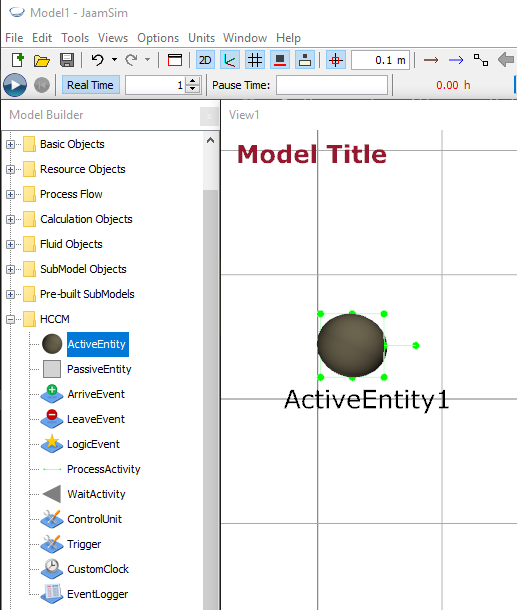
\includegraphics[width=\textwidth,height=75mm]{chapters/clinic_1/figures/entity_creation.png}

}

\caption{\label{fig-ent_pic}Screenshot of an ActiveEntity}

\end{marginfigure}%

Repeat this process two more times and create ActiveEntities called
\textbf{ReceptionistEntity} and \textbf{CTMachineEntity}.

An ActiveEntity object by itself does not create any entities in the
simulation, it just acts as a prototype for entities. To create entities
an ArriveEvent object is used, which simulates
patients/receptionists/CTMachines arriving at the clinic. The
ArriveEvent object creates a series of entities that are passed to the
next object in a process. The PrototypeEntity keyword identifies the
entity to be copied. The rate at which entities are generated is
determined by the InterArrivalTime and FirstArrivalTime keywords. Create
three ArriveEvents called \textbf{PatientArrival},
\textbf{ReceptionistArrival}, and \textbf{CTMachineArrival}, and set the
PrototypeEntity to be the related entity (patient, receptionist,
CTMachine).

We also need to create objects that represent the entities leaving,
called LeaveEvent, we will only create one for the patients, as we are
assuming that the receptionist and CT machines are available 24/7 so
they do not need to leave. Drag and drop a leave event into the
simulation, rename it \textbf{PatientLeave}, and set the Participant to
be the patient entity (under the HCCM tab).

The patients waiting for check in and scanning, and both the
receptionist and CT machines waiting for tasks can be represented by
WaitActivities, so create four WaitActivities and rename them
\textbf{WaitForCheckIn}, \textbf{WaitForScan},
\textbf{WaitForTaskReceptionist}, and \textbf{WaitForTaskCTMachine}
respectively, and once again set the Participant to the respective
entity.

We can then represent the patient doing check in with the receptionist,
and the patient being scanned by a CT machine as process activities.
Create two process activities and rename them \textbf{CheckIn}, and
\textbf{Scan}.

We also need to create objects to represent the probability
distributions that the interarrival, check in, and scan times come from.
Probability distributions can be represented in Jaamsim with
distribution objects. If we examine the PatientArrival object we see two
keywords FirstArrivalTime and InterArrivalTime which determine the rate
that the entities are created. For a Poisson process with an average of
8 arrivals per hour the interarrival times can be modelled by an
exponential distribution with mean 0.125 hours. We therefore go into the
Probability Distributions palette in the Model Builder window and create
an ExponentialDistribution object and name it
\textbf{ArrivalDistribution}. First we set the UnitType keyword to be
\textbf{TimeUnit}, then we set the mean of the distribution to
\textbf{0.125 h}. The UnitType tells Jaamsim what type of value we want
the distribution object to create, in our case this is the time between
arrivals in hours, which is a unit of time. Also make sure that the
\textbf{RandomSeed} is 1, this determines the seed for the random number
generator. Table~\ref{tbl-arr_dist} shows the keywords and values for
the \textbf{ArrivalDistribution} object.

\begin{table}

\caption{\label{tbl-arr_dist}Arrival Distribution Inputs}

\centering{

\begin{tabular}{@{}lll@{}}
\toprule
Object                & Keyword         & Value         \\ \midrule
ArrivalDistribution   & UnitType        & TimeUnit      \\
                      & RandomSeed      & 1             \\
                      & Mean            & 0.125 h       \\ \bottomrule
\end{tabular}

}

\end{table}%

We need to repeat these steps for the check in and scan processes, which
follow uniform and log-normal distributions respectively, so create a
UniformDistribution object called \textbf{CheckInDistribution} and a
\textbf{LogNormalDistribution} object called \textbf{ScanDistribution}.
Then update the keywords of the distribution objects as follows in
Table~\ref{tbl-serv_dists}:

\begin{table}

\caption{\label{tbl-serv_dists}Check In and Scan Distributions}

\centering{

\begin{tabular}{@{}lll@{}}
\toprule
Object              & Keyword     & Value                       \\ \midrule
CheckInDistribtuion & UnitType    & TimeUnit                    \\
                    & RandomSeed  & 2                           \\
                    & MinValue    & 2 min                       \\
                    & MaxValue    & 5 min                       \\
 & & \\
ScanDistribution    & UnitType    & TimeUnit                    \\
                    & RandomSeed  & 3                           \\
                    & Scale       & 1 h                         \\
                    & NormalMean  & -1.34                       \\
                    & NormalSD    & 0.29                        \\ \bottomrule
\end{tabular}

}

\end{table}%

The final object we need at this stage is a Statistics object, to
capture some output about the patients. This is found under the
ProcessFlow palette, create a Statistics object and call it
\textbf{TimeInSystem}.

At this point you should have the objects shown in
Table~\ref{tbl-mod_objs} in your simulation.

\begin{table}

\caption{\label{tbl-mod_objs}Model Objects}

\centering{

\begin{tabular}{@{}ll@{}}
\toprule
Object Type     & Name             \\ \midrule
ActiveEntity    & PatientEntity    \\
ActiveEntity    & ReceptionistEntity    \\
ActiveEntity    & CTMachineEntity  \\
                &                  \\
ArriveEvent     & PatientArrival   \\
ArriveEvent     & ReceptionistArrival   \\
ArriveEvent     & CTMachineArrival \\
                &                  \\
LeaveEvent      & PatientLeave     \\
                &                  \\
WaitActivity    & WaitForCheckIn   \\
WaitActivity    & WaitForScan      \\
WaitActivity    & WaitForTaskReceptionist \\
WaitActivity    & WaitForTaskCTMachine    \\
                &                  \\
ProcessActivity & CheckIn          \\
ProcessActivity & Scan             \\
                &                  \\
ExponentialDistribution & ArrivalDistribution             \\
UniformDistribution & CheckInDistribution             \\
LogNormalDistribution & ScanDistribution             \\
                &                  \\
Statistics      & TimeInSystem   \\ \bottomrule
\end{tabular}

}

\end{table}%

Once you have created all of these objects lay them out similarly to as
shown in Figure~\ref{fig-sim_pic}.

\begin{figure*}[htbp]

\centering{

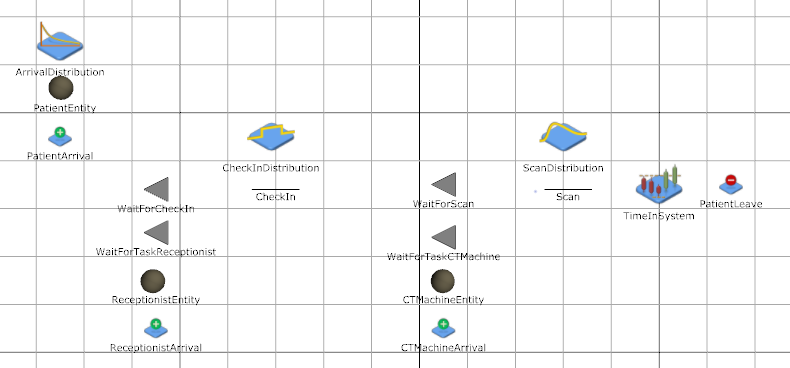
\includegraphics{chapters/clinic_1/figures/Example_layout_2.png}

}

\caption{\label{fig-sim_pic}Screenshot of Simulation Model Layout}

\end{figure*}%

Create a new folder in the \textbf{labs} folder called \textbf{RC1} and
save your simulation as \textbf{radiology\_lab.cfg} or something similar
inside the new folder. Also take this opportunity to change the graphics
of the PatientEntity, ReceptionistEntity and CTMachineEntity. Download
the patient.png, receptionist.png, and ctscanner.png (icons made by
Freepik from www.flaticon.com) files from Canvas and save them in the
same folder as your simulation .cfg file. Then in Jaamsim right click on
PatientEntity and select Change Graphics. Click on Import and navigate
to your downloaded patient.png, import it (it may be called
patient-model) and accept the change. Repeat the process for the
receptionists, and CT scanners.

\subsection{Configuring Objects}\label{configuring-objects}

Now that we have created the objects we need, we need to set the options
for the each of them, starting with the ArriveEvents. The PatientArrival
should have both the first arrival time and inter arrival times set by
the ArrivalDistribution object, use the PatientEntity as a prototype,
and the NextAEJObject should be WaitForCheckIn. NextAEJObject stands for
next activity/event/Jaamsim object and refers to the fact that the next
place an entity goes could be a standard Jaamsim object or a custom HCCM
activity or event. For the arrive events we set NextAEJObject to the
object that represents the activity that is transitioned to at the end
of the event state changes in the conceptual model. For the
ReceptionistArrival and CTMachineArrival we need to: set the prototype
entity; both MaxNumber and InitialNumber (1 for receptionist, 3 for CT
Machine); and set the NextAEJObject to the respective wait activity.

\begin{table}

\caption{\label{tbl-arr_params}Arrival Event Parameters}

\centering{

\begin{tabular}{@{}llll@{}}
\toprule
Object              & Tab        & Keyword         & Value         \\ \midrule
PatientArrival      & Key Inputs & PrototypeEntity  & PatientEntity \\
PatientArrival      & Key Inputs & FirstArrivalTime & ArrivalDistribution \\
PatientArrival      & Key Inputs & InterArrivalTime & ArrivalDistribution \\
PatientArrival      & HCCM       & NextAEJObject    & WaitForCheckIn \\
                    &            &                  &                 \\
ReceptionistArrival & Key Inputs & PrototypeEntity  & ReceptionistEntity \\
ReceptionistArrival & Key Inputs & MaxNumber        & 1               \\
ReceptionistArrival & Key Inputs & InitialNumber        & 1               \\
ReceptionistArrival & HCCM       & NextAEJObject    & WaitForTaskReceptionist \\
                    &            &                  &                 \\
CTMachineArrival    & Key Inputs & PrototypeEntity  & CTMachineEntity \\
CTMachineArrival    & Key Inputs & MaxNumber        & 3               \\
CTMachineArrival    & Key Inputs & InitialNumber        & 3               \\
CTMachineArrival    & HCCM       & NextAEJObject    & WaitForTaskCTMachine \\ \bottomrule
\end{tabular}

}

\end{table}%

Next we will set the options for the Process Activities (and Statistics)
so that the routing/flow for the entities is correct. The Check In
activity has both the Patient and Receptionist as participants so we set
the Participant list to PatientEntity, ReceptionistEntity. The duration
is determined by the check in distribution, so we just set the duration
to be CheckInDistribution object. After Check In the Patient starts
waiting for a scan and the receptionist goes back to waiting for a task,
so we set the NextAEJList to WaitForScan, WaitForTaskReceptionist. The
Scan activity has both the Patient and CTMachine as participants and the
duration is determined by the ScanDistribution object. After Scan the
Patient should just leave, but we want to record some statistics first
so we send it to TimeInSystem, and the CTMachine goes back to
WaitForTaskCTMachine. For Process Activities the NextAEJList is similar
to the NextAEJObject from the Arrive Events (which is similar to
NextComponent), the difference is that a list of next objects is given,
one for each of the participants in the activity. The participants are
sent to the corresponding element of the list so it is important that
the next activities are in the same order as the participants.

Note that when you click on the checkboxes in the popup menu for both
ParticipantList and NextAEJList the items are added in alphabetical
order, not the order you click them in. This is particularly important
for the Scan activity as the CTMachineEntity comes before the
PatientEntity alphabetically, but for the next activities TimeInSystem
is before WaitForTaskCTMachine alphabetically so the two lists will not
be in the same order.

\begin{table}

\caption{\label{tbl-pro_params}Process Activity Parameters}

\centering{

\begin{tabular}{@{}llll@{}}
\toprule
Object              & Tab        & Keyword          & Value         \\ \midrule
CheckIn             & Key Inputs & Duration         & CheckInDistribution \\
CheckIn             & HCCM       & ParticipantList  & PatientEntity ReceptionistEntity \\
CheckIn             & HCCM       & NextAEJList      & WaitForScan WaitForTaskReceptionist   \\
                    &            &                  &                 \\
Scan                & Key Inputs & Duration         & ScanDistribution \\
Scan                & HCCM       & ParticipantList  & PatientEntity CTMachineEntity \\
Scan                & HCCM       & NextAEJList      & TimeInSystem WaitForTaskCTMachine   \\\bottomrule
\end{tabular}

}

\end{table}%

The last object we need to configure before the simulation will run (it
will run but it will not quite work correctly) is the TimeInSystem
object. This is a Statistics object which collects a value from each
Entity that passes through it and outputs the mean of the sampled
values. We then need to finish the routing so that patients leave after
going through the TimeInSystem, and tell the Statistics object which
value to record as shown in Table~\ref{tbl-stats}, note that
\textbf{this} refers to the Statistics object itself, \textbf{obj}
refers to the entity that the Statistics object is currently processing,
and \textbf{TotalTime} is an output on the entity that stores the total
time that the entity has been in the simulation for.

\begin{table}

\caption{\label{tbl-stats}Collecting Statistics}

\centering{

\begin{tabular}{@{}lll@{}}
\toprule
Object        & Keyword        & Value \\ \midrule
TimeInSystem  & NextComponent  & PatientLeave  \\
              & UnitType       & TimeUnit   \\ 
              & SampleValue    & this.obj.TotalTime  \\ \bottomrule
\end{tabular}

}

\end{table}%

Save your simulation again. If you run your simulation now you should
see one receptionist arrive and wait, three CT machines arrive and wait,
and patients arrive, and wait for check in. However nothing else will
happen and all of the entities will simply be waiting, this is because
we have not specified any logic to be triggered when the entities start
waiting.

\section{Model Logic -- Java}\label{model-logic-java}

In your VSCode project you should have a folder called
\textbf{sim\_custom} under the Explorer tab on the left-hand side in
VSCode. First right-click on this folder and select New Java Package.
Enter \textbf{labs} for the name of the package and press Enter.

\begin{figure}[htbp]

\centering{

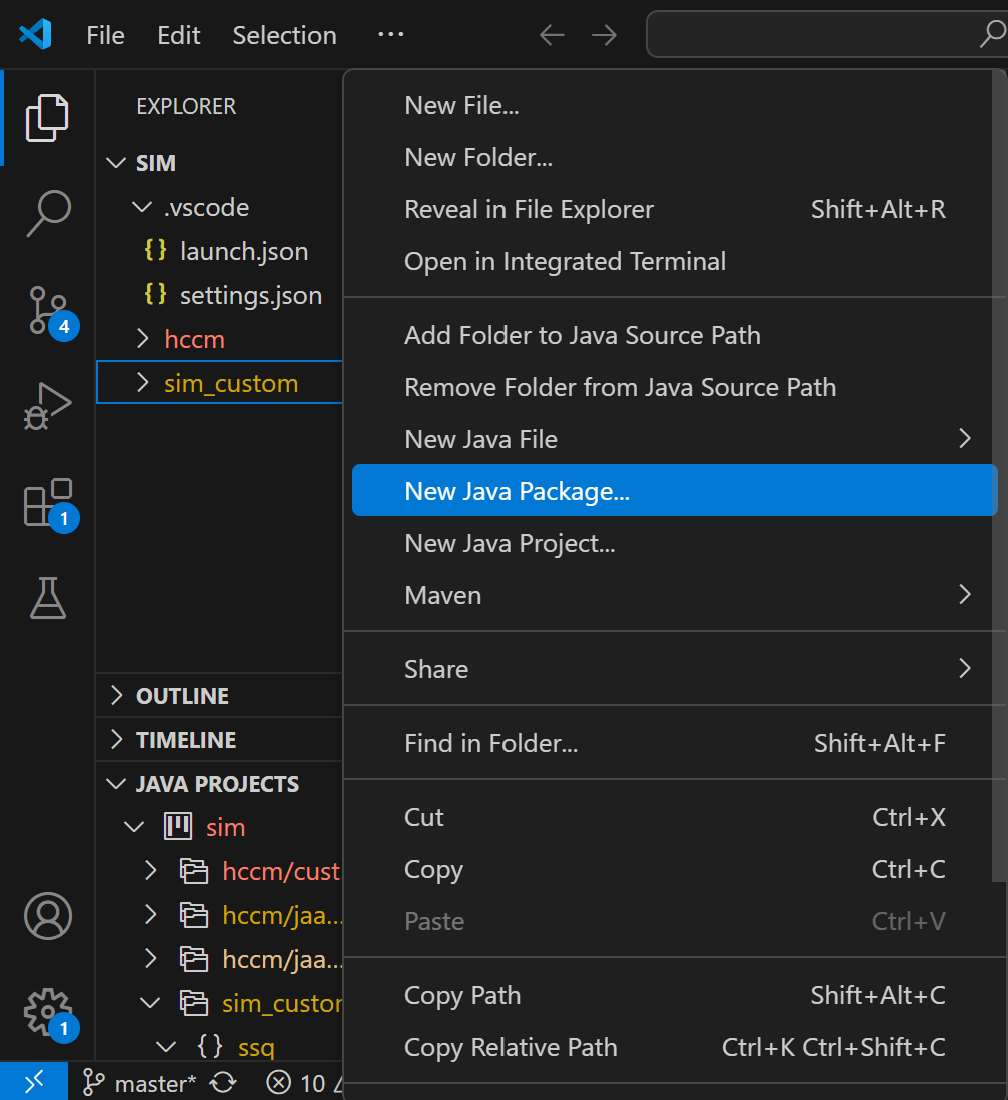
\includegraphics{chapters/clinic_1/figures/vscode_package_creation_1.png}

}

\caption{\label{fig-create_package_1}First Step in Creating a New
Package}

\end{figure}%

\begin{figure*}[htbp]

\centering{

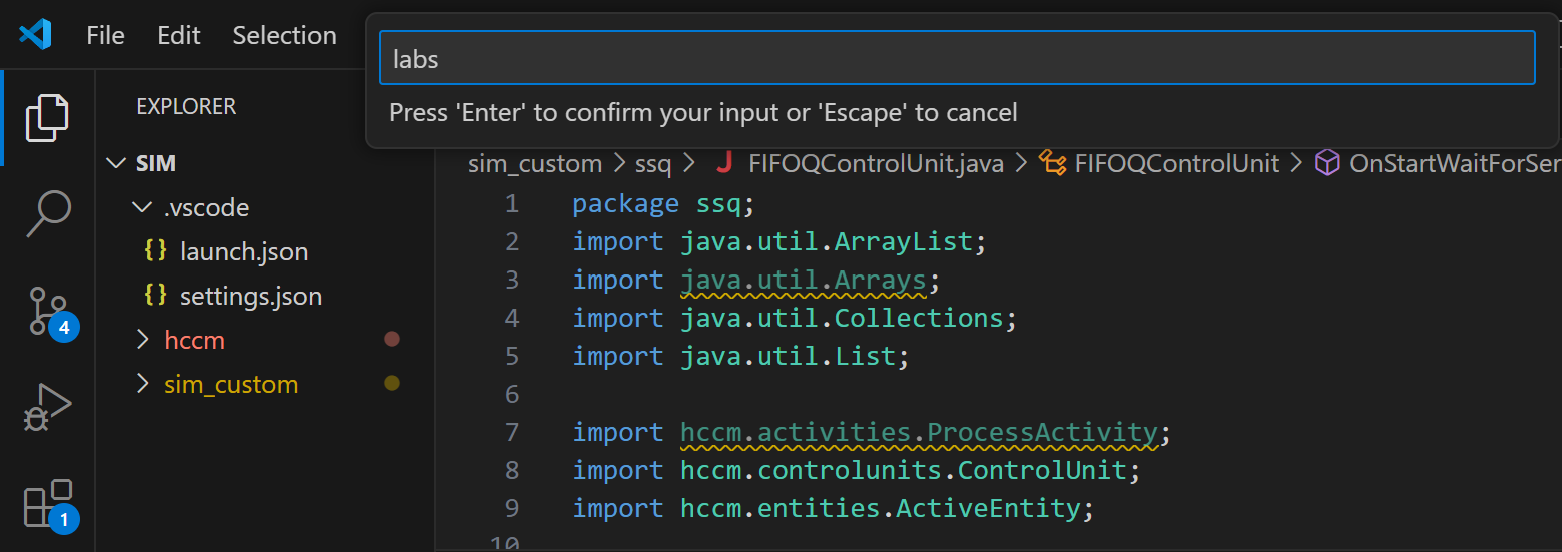
\includegraphics{chapters/clinic_1/figures/vscode_package_creation_2.png}

}

\caption{\label{fig-create_package_2}Second Step in Creating a New
Package}

\end{figure*}%

A new folder called \textbf{labs} should have been created within the
\textbf{sim\_custom} folder. Right click on the newly created
\textbf{labs} folder and select New Java File \(\rightarrow\) Class.
Name the Class \textbf{RadiologyControlUnit} and press Enter.

\begin{figure}[htbp]

\centering{

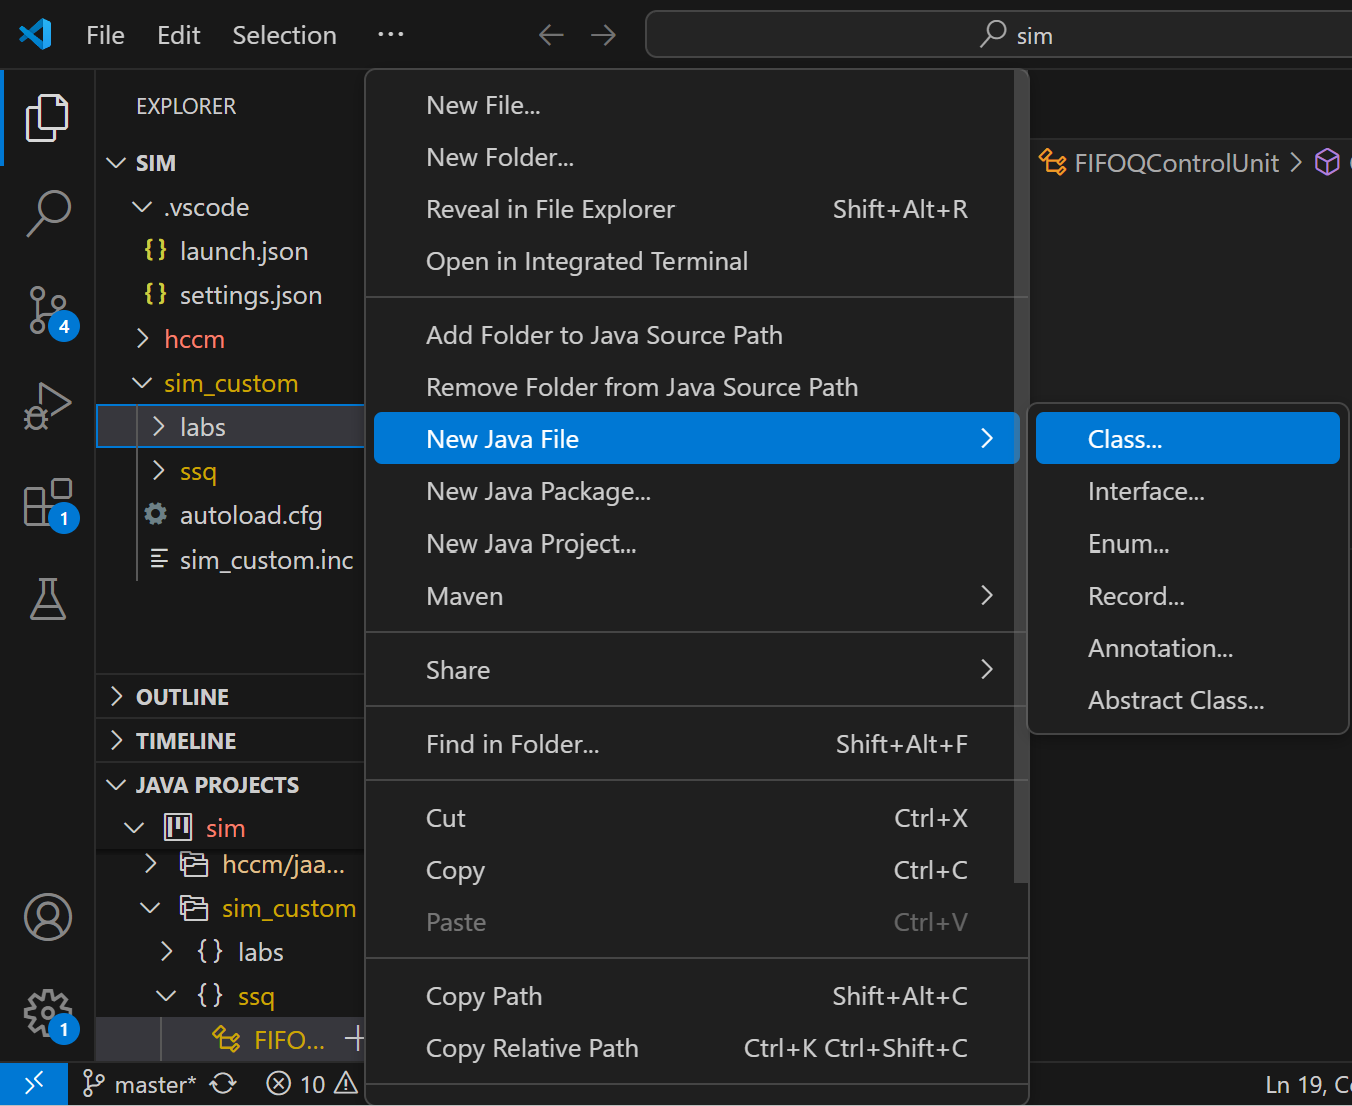
\includegraphics{chapters/clinic_1/figures/vscode_class_creation_1.png}

}

\caption{\label{fig-create_class_1}First Step in Creating a New Class}

\end{figure}%

\begin{figure*}[htbp]

\centering{

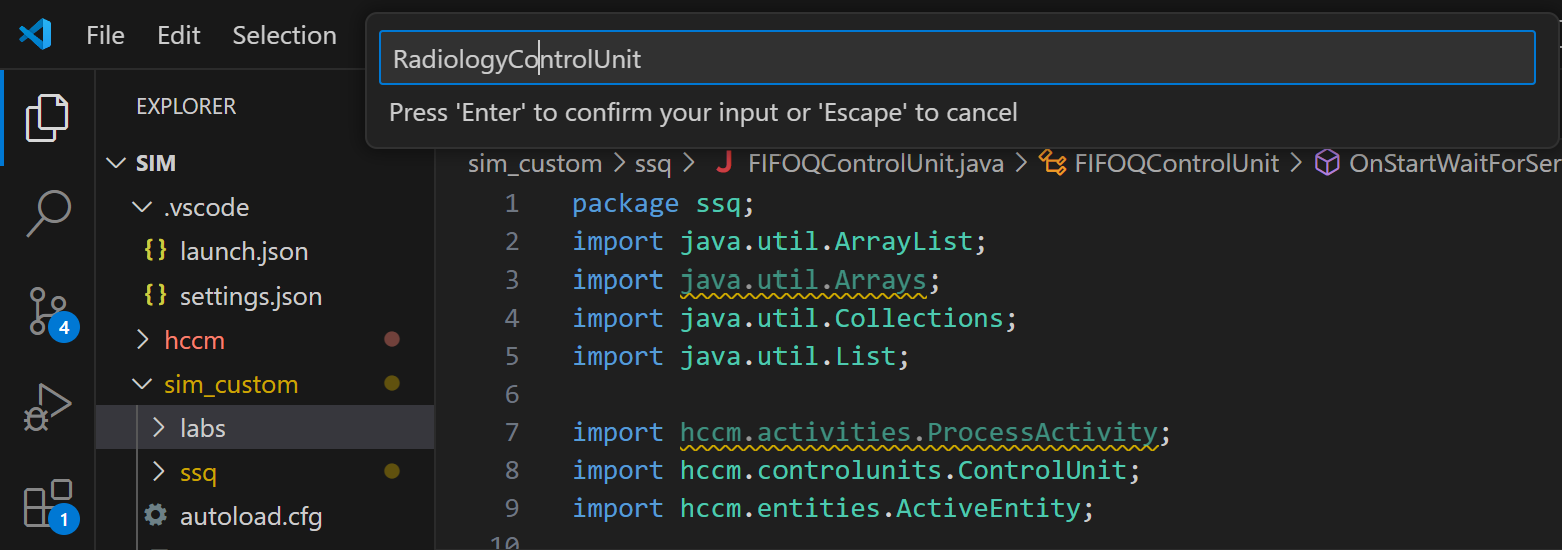
\includegraphics{chapters/clinic_1/figures/vscode_class_creation_2.png}

}

\caption{\label{fig-create_class_2}Second Step in Creating a New Class}

\end{figure*}%

\newpage{}

The final step required to make this new object available in the
simulation is to add to the contents of the sim\_custom.inc file that we
put in sim \(\rightarrow\) hccm \(\rightarrow\) jaamsim \(\rightarrow\)
src \(\rightarrow\) main \(\rightarrow\) resources \(\rightarrow\)
resources \(\rightarrow\) inputs. There should already be some code
there from the previous lab, so you only need to add lines 3, 7, and 10.
If you want to copy and paste this make sure the quotes are copied
correctly and the returns (arrows) are removed. Alternatively there is a
new sim\_custom.inc file here XXX on Canvas under Jaamsim Lab 1 that you
can use directly.

\begin{Shaded}
\begin{Highlighting}[numbers=left,,]
\NormalTok{Define ObjectType \{}
\NormalTok{    FIFOQControlUnit}
\NormalTok{    RadiologyControlUnit}
\NormalTok{\}}

\NormalTok{ControllerIconModel ImageFile \{ \textquotesingle{}\textless{}res\textgreater{}/images/Controller{-}256.png\textquotesingle{} \}  Transparent \{ TRUE \}}
\NormalTok{AssembleIconModel ImageFile \{ \textquotesingle{}\textless{}res\textgreater{}/images/Assemble{-}256.png\textquotesingle{} \}  Transparent \{ TRUE \}}

\NormalTok{FIFOQControlUnit JavaClass \{ ssq.FIFOQControlUnit \}  Palette \{ \textquotesingle{}Single Server Queue\textquotesingle{} \} DefaultDisplayModel \{ ControllerIconModel \} IconFile \{ \textquotesingle{}\textless{}res\textgreater{}/images/Controller{-}24.png\textquotesingle{} \} DefaultSize \{ 0.5 0.5 0.5 m \}}
\NormalTok{RadiologyControlUnit JavaClass \{ labs.RadiologyControlUnit \}  Palette \{ \textquotesingle{}Custom Logic\textquotesingle{} \} DefaultDisplayModel \{ AssembleIconModel \} IconFile \{ \textquotesingle{}\textless{}res\textgreater{}/images/Assemble{-}24.png\textquotesingle{} \} DefaultSize \{ 0.5 0.5 0.5 m \}}
\end{Highlighting}
\end{Shaded}

Once you have updated the sim\_custom.inc file, restart Jaamsim. If
everything is working correctly the RadiologyControlUnit object should
now be available under the Custom Logic palette as shown in the
screenshot below:

\begin{figure}[htbp]

\centering{

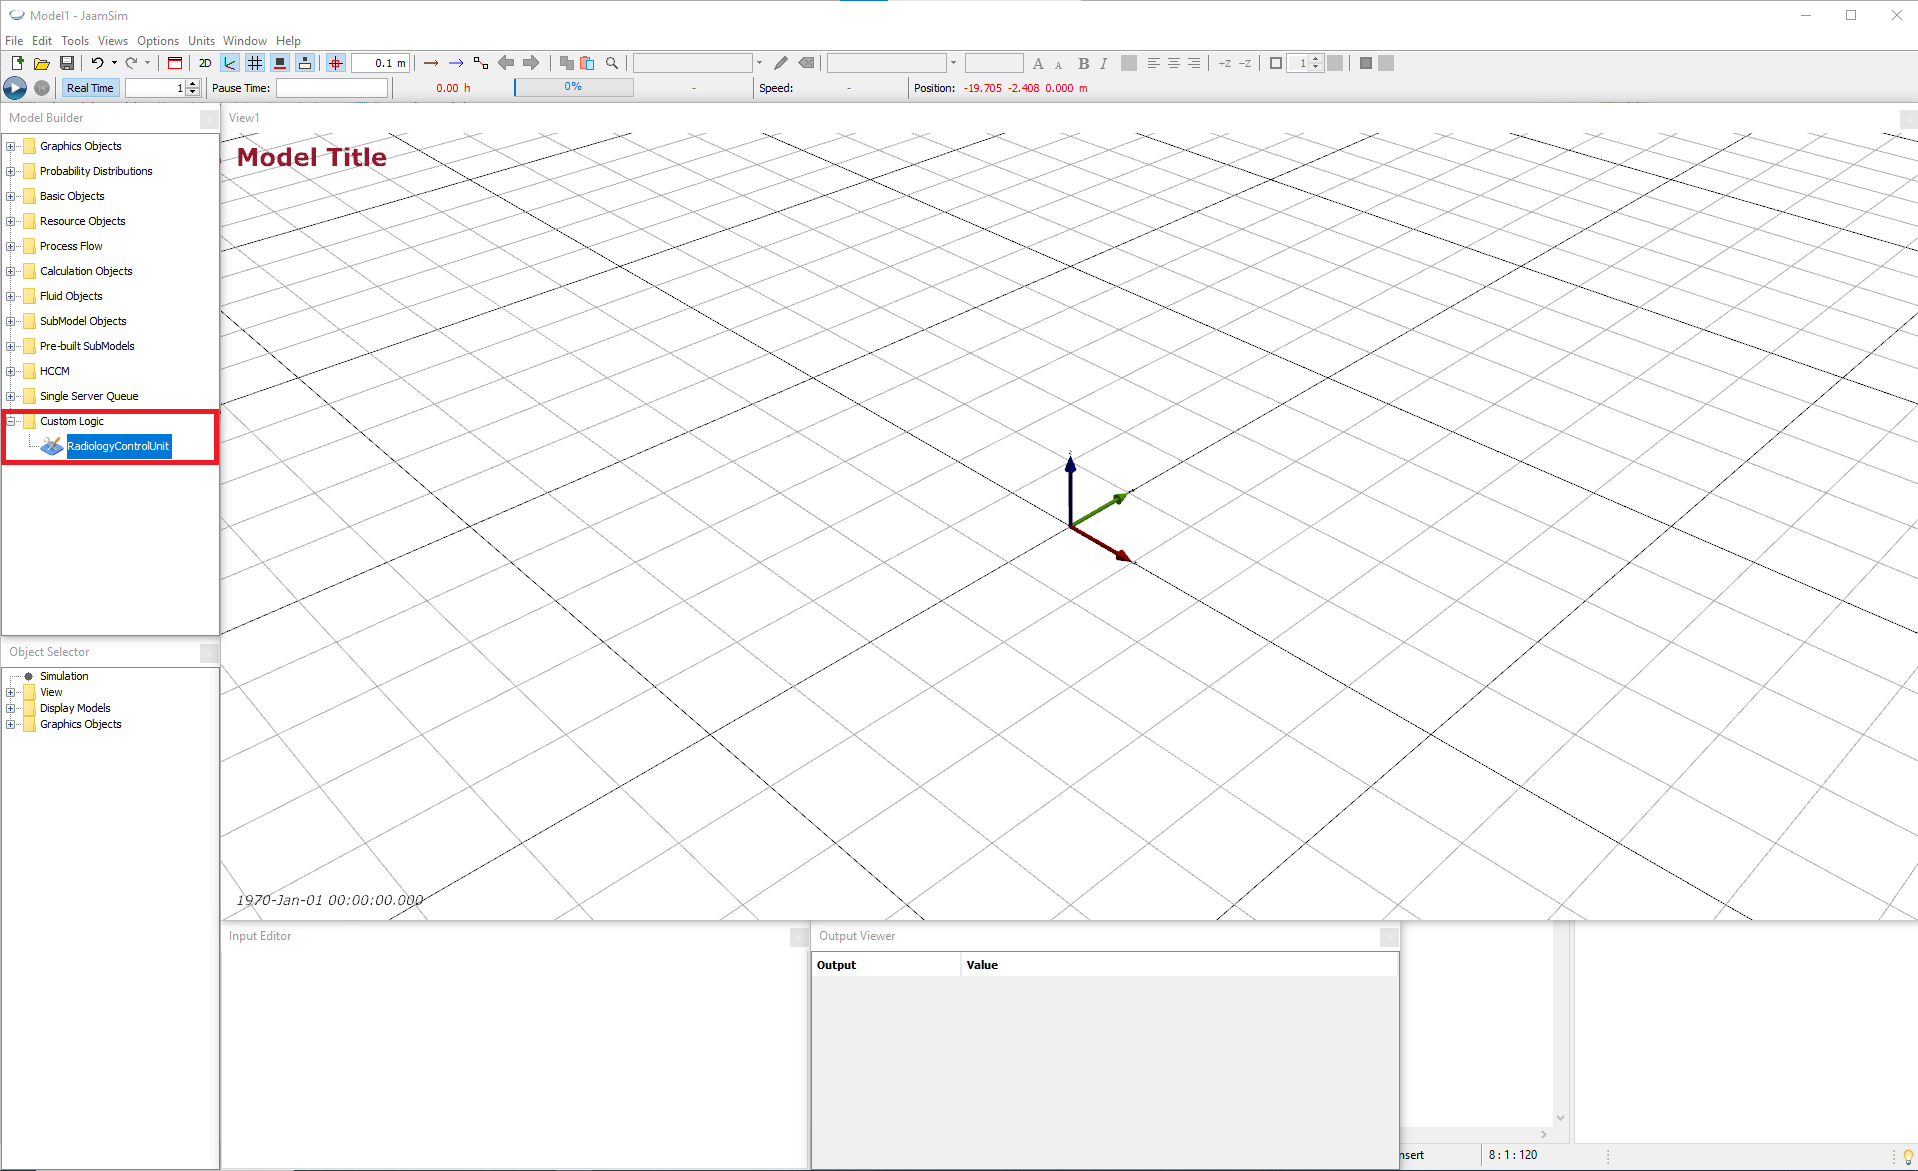
\includegraphics{chapters/clinic_1/figures/control_unit_jaamsim_2.png}

}

\caption{\label{fig-cu_obj}Screenshot of Control Unit Object}

\end{figure}%

Once you have the new RadiologyControlUnit object available open your
simulation and create one.

We now need to add the Java code to the new RadiologyControlUnit class
to run the control policies. First add the following imports under the
package declaration. \textbf{Note} These code snippets for this lab are
provided in a separate file for you here XXX.

\begin{Shaded}
\begin{Highlighting}[numbers=left,,]
\KeywordTok{package}\ImportTok{ labs}\OperatorTok{;}
\KeywordTok{import} \ImportTok{java}\OperatorTok{.}\ImportTok{util}\OperatorTok{.}\ImportTok{ArrayList}\OperatorTok{;}
\KeywordTok{import} \ImportTok{java}\OperatorTok{.}\ImportTok{util}\OperatorTok{.}\ImportTok{Arrays}\OperatorTok{;}
\KeywordTok{import} \ImportTok{java}\OperatorTok{.}\ImportTok{util}\OperatorTok{.}\ImportTok{Collections}\OperatorTok{;}
\KeywordTok{import} \ImportTok{java}\OperatorTok{.}\ImportTok{util}\OperatorTok{.}\ImportTok{List}\OperatorTok{;}

\KeywordTok{import} \ImportTok{hccm}\OperatorTok{.}\ImportTok{activities}\OperatorTok{.}\ImportTok{ProcessActivity}\OperatorTok{;}
\KeywordTok{import} \ImportTok{hccm}\OperatorTok{.}\ImportTok{controlunits}\OperatorTok{.}\ImportTok{ControlUnit}\OperatorTok{;}
\KeywordTok{import} \ImportTok{hccm}\OperatorTok{.}\ImportTok{entities}\OperatorTok{.}\ImportTok{ActiveEntity}\OperatorTok{;}
\end{Highlighting}
\end{Shaded}

Then, within the definition of the class we need to create four methods
that represent the four control policies in the model. Each control
policy is a public method of the class that does not return any value
(is void) and takes both a list of Active Entities, and the simulation
time as inputs. We will use the same names for the methods as the
control policies in the conceptual model:
\textbf{OnStartWaitForCheckIn}, \textbf{OnStartWaitForScan},
\textbf{OnStartWaitForTaskReceptionist}, and
\textbf{OnStartWaitForTaskCTMachine}. In the first of these,
\textbf{OnStartWaitForCheckIn} we first need to get a list of the
Receptionist Entities that are currently in the
'\,'WaitForTaskReceptionist'' activity, and we also create a comparator
object that is used to sort a list of entities by when they started
their current activity.

Once we have the list of idle receptionists we check whether it is not
empty, and if it isn't proceed to sort it, select the first one, and
transition the patient and receptionist to the check in activity.

\begin{figure*}

\begin{codebox}

\begin{Shaded}
\begin{Highlighting}[numbers=left,,]
\KeywordTok{public} \DataTypeTok{void} \FunctionTok{OnStartWaitForCheckIn}\OperatorTok{(}\BuiltInTok{List}\OperatorTok{\textless{}}\NormalTok{ActiveEntity}\OperatorTok{\textgreater{}}\NormalTok{ ents}\OperatorTok{,} \DataTypeTok{double}\NormalTok{ simTime}\OperatorTok{)} \OperatorTok{\{}
        
    \BuiltInTok{ArrayList}\OperatorTok{\textless{}}\NormalTok{ActiveEntity}\OperatorTok{\textgreater{}}\NormalTok{ idleReceps }\OperatorTok{=} \KeywordTok{this}\OperatorTok{.}\FunctionTok{getEntitiesInActivity}\OperatorTok{(}\StringTok{"ReceptionistEntity"}\OperatorTok{,} \StringTok{"WaitForTaskReceptionist"}\OperatorTok{,}\NormalTok{ simTime}\OperatorTok{);}
\NormalTok{    ActivityStartCompare actSartComp }\OperatorTok{=} \KeywordTok{this}\OperatorTok{.}\FunctionTok{new} \FunctionTok{ActivityStartCompare}\OperatorTok{();}        
    
    \ControlFlowTok{if} \OperatorTok{(}\NormalTok{idleReceps}\OperatorTok{.}\FunctionTok{size}\OperatorTok{()} \OperatorTok{\textgreater{}} \DecValTok{0}\OperatorTok{)} \OperatorTok{\{}
      \BuiltInTok{Collections}\OperatorTok{.}\FunctionTok{sort}\OperatorTok{(}\NormalTok{idleReceps}\OperatorTok{,}\NormalTok{ actSartComp}\OperatorTok{);}
      
\NormalTok{      ActiveEntity patient }\OperatorTok{=}\NormalTok{ ents}\OperatorTok{.}\FunctionTok{get}\OperatorTok{(}\DecValTok{0}\OperatorTok{);}
\NormalTok{      ActiveEntity receptionist }\OperatorTok{=}\NormalTok{ idleReceps}\OperatorTok{.}\FunctionTok{get}\OperatorTok{(}\DecValTok{0}\OperatorTok{);}
      
      \FunctionTok{transitionTo}\OperatorTok{(}\StringTok{"CheckIn"}\OperatorTok{,}\NormalTok{ patient}\OperatorTok{,}\NormalTok{ receptionist}\OperatorTok{);}
    \OperatorTok{\}}
  \OperatorTok{\}}
\end{Highlighting}
\end{Shaded}

\end{codebox}

\end{figure*}%

Similar methods are defined for the other control policies, with small
changes based on the types of entities that are being checked, and the
activity that is started. There are gaps that need to be filled in on
lines 3, 24, and 42. In the first gap you need to create an array that
contains all of the CT Machines that are currently idle. In the second,
you need to select which of the patients that are currently waiting
should do check in with the receptionist. In the third, you need to
start the next activity with the patient and CT Machine. All of these
have similar lines in the first method that you can use as a guide.

\begin{figure*}

\begin{codebox}

\begin{Shaded}
\begin{Highlighting}[numbers=left,,]
\KeywordTok{public} \DataTypeTok{void} \FunctionTok{OnStartWaitForScan}\OperatorTok{(}\BuiltInTok{List}\OperatorTok{\textless{}}\NormalTok{ActiveEntity}\OperatorTok{\textgreater{}}\NormalTok{ ents}\OperatorTok{,} \DataTypeTok{double}\NormalTok{ simTime}\OperatorTok{)} \OperatorTok{\{}
  
    \CommentTok{// A //}
\NormalTok{    ActivityStartCompare actSartComp }\OperatorTok{=} \KeywordTok{this}\OperatorTok{.}\FunctionTok{new} \FunctionTok{ActivityStartCompare}\OperatorTok{();}        
    
    \ControlFlowTok{if} \OperatorTok{(}\NormalTok{idleCTs}\OperatorTok{.}\FunctionTok{size}\OperatorTok{()} \OperatorTok{\textgreater{}} \DecValTok{0}\OperatorTok{)} \OperatorTok{\{}
      \BuiltInTok{Collections}\OperatorTok{.}\FunctionTok{sort}\OperatorTok{(}\NormalTok{idleCTs}\OperatorTok{,}\NormalTok{ actSartComp}\OperatorTok{);}
      
\NormalTok{      ActiveEntity patient }\OperatorTok{=}\NormalTok{ ents}\OperatorTok{.}\FunctionTok{get}\OperatorTok{(}\DecValTok{0}\OperatorTok{);}
\NormalTok{      ActiveEntity ct }\OperatorTok{=}\NormalTok{ idleCTs}\OperatorTok{.}\FunctionTok{get}\OperatorTok{(}\DecValTok{0}\OperatorTok{);}

      \FunctionTok{transitionTo}\OperatorTok{(}\StringTok{"Scan"}\OperatorTok{,}\NormalTok{ patient}\OperatorTok{,}\NormalTok{ ct}\OperatorTok{);}
    \OperatorTok{\}}
  \OperatorTok{\}}
    
\KeywordTok{public} \DataTypeTok{void} \FunctionTok{OnStartWaitForTaskReceptionist}\OperatorTok{(}\BuiltInTok{List}\OperatorTok{\textless{}}\NormalTok{ActiveEntity}\OperatorTok{\textgreater{}}\NormalTok{ ents}\OperatorTok{,} \DataTypeTok{double}\NormalTok{ simTime}\OperatorTok{)} \OperatorTok{\{}
      
  \BuiltInTok{ArrayList}\OperatorTok{\textless{}}\NormalTok{ActiveEntity}\OperatorTok{\textgreater{}}\NormalTok{ waitPats }\OperatorTok{=} \KeywordTok{this}\OperatorTok{.}\FunctionTok{getEntitiesInActivity}\OperatorTok{(}\StringTok{"PatientEntity"}\OperatorTok{,} \StringTok{"WaitForCheckIn"}\OperatorTok{,}\NormalTok{ simTime}\OperatorTok{);}
\NormalTok{  ActivityStartCompare actSartComp }\OperatorTok{=} \KeywordTok{this}\OperatorTok{.}\FunctionTok{new} \FunctionTok{ActivityStartCompare}\OperatorTok{();}
  
  \ControlFlowTok{if} \OperatorTok{(}\NormalTok{waitPats}\OperatorTok{.}\FunctionTok{size}\OperatorTok{()} \OperatorTok{\textgreater{}} \DecValTok{0}\OperatorTok{)} \OperatorTok{\{}
    \BuiltInTok{Collections}\OperatorTok{.}\FunctionTok{sort}\OperatorTok{(}\NormalTok{waitPats}\OperatorTok{,}\NormalTok{ actSartComp}\OperatorTok{);}
    
    \CommentTok{// B //}
\NormalTok{    ActiveEntity receptionist }\OperatorTok{=}\NormalTok{ ents}\OperatorTok{.}\FunctionTok{get}\OperatorTok{(}\DecValTok{0}\OperatorTok{);}

    \FunctionTok{transitionTo}\OperatorTok{(}\StringTok{"CheckIn"}\OperatorTok{,}\NormalTok{ patient}\OperatorTok{,}\NormalTok{ receptionist}\OperatorTok{);}
  \OperatorTok{\}}
\OperatorTok{\}}

\KeywordTok{public} \DataTypeTok{void} \FunctionTok{OnStartWaitForTaskCTMachine}\OperatorTok{(}\BuiltInTok{List}\OperatorTok{\textless{}}\NormalTok{ActiveEntity}\OperatorTok{\textgreater{}}\NormalTok{ ents}\OperatorTok{,} \DataTypeTok{double}\NormalTok{ simTime}\OperatorTok{)} \OperatorTok{\{}
  
  \BuiltInTok{ArrayList}\OperatorTok{\textless{}}\NormalTok{ActiveEntity}\OperatorTok{\textgreater{}}\NormalTok{ waitPats }\OperatorTok{=} \KeywordTok{this}\OperatorTok{.}\FunctionTok{getEntitiesInActivity}\OperatorTok{(}\StringTok{"PatientEntity"}\OperatorTok{,} \StringTok{"WaitForScan"}\OperatorTok{,}\NormalTok{ simTime}\OperatorTok{);}
\NormalTok{  ActivityStartCompare actSartComp }\OperatorTok{=} \KeywordTok{this}\OperatorTok{.}\FunctionTok{new} \FunctionTok{ActivityStartCompare}\OperatorTok{();}        
    
  \ControlFlowTok{if} \OperatorTok{(}\NormalTok{waitPats}\OperatorTok{.}\FunctionTok{size}\OperatorTok{()} \OperatorTok{\textgreater{}} \DecValTok{0}\OperatorTok{)} \OperatorTok{\{}
    \BuiltInTok{Collections}\OperatorTok{.}\FunctionTok{sort}\OperatorTok{(}\NormalTok{waitPats}\OperatorTok{,}\NormalTok{ actSartComp}\OperatorTok{);}
    
\NormalTok{    ActiveEntity patient }\OperatorTok{=}\NormalTok{ waitPats}\OperatorTok{.}\FunctionTok{get}\OperatorTok{(}\DecValTok{0}\OperatorTok{);}
\NormalTok{    ActiveEntity ct }\OperatorTok{=}\NormalTok{ ents}\OperatorTok{.}\FunctionTok{get}\OperatorTok{(}\DecValTok{0}\OperatorTok{);}

    \CommentTok{// C //}
  \OperatorTok{\}}
\OperatorTok{\}}
\end{Highlighting}
\end{Shaded}

\end{codebox}

\end{figure*}%

The final step needed to get this logic into the simulation is to define
Triggers that initiate these methods and where/when they should be
called. To do this create four Trigger objects, called
\textbf{StartWaitCheckIn}, \textbf{StartWaitScan},
\textbf{StartWaitTaskReceptionist}, and \textbf{StartWaitTaskCTMachine}
from the HCCM palette and set the ControlUnit and ControlPolicy for each
one. The value of the ControlPolicy keyword needs to exactly match the
name of the method you have defined in the java code.

\begin{table}

\caption{\label{tbl-trig_params}Trigger Parameters}

\centering{

\begin{tabular}{@{}llll@{}}
\toprule
Object                    & Tab  & Keyword       & Value         \\ \midrule
StartWaitCheckIn          & HCCM & ControlUnit   & RadiologyControlUnit1 \\
StartWaitCheckIn          & HCCM & ControlPolicy & OnStartWaitForCheckIn \\
                          &      &               &                 \\
StartWaitScan             & HCCM & ControlUnit   & RadiologyControlUnit1 \\
StartWaitScan             & HCCM & ControlPolicy & OnStartWaitForScan \\
                          &      &               &                 \\
StartWaitTaskReceptionist & HCCM & ControlUnit   & RadiologyControlUnit1 \\
StartWaitTaskReceptionist & HCCM & ControlPolicy & OnStartWaitForTaskReceptionist \\
                    &            &                  &                 \\
StartWaitTaskCTMachine    & HCCM & ControlUnit   & RadiologyControlUnit1 \\
StartWaitTaskCTMachine    & HCCM & ControlPolicy & OnStartWaitForTaskCTMachine \\
\bottomrule
\end{tabular}

}

\end{table}%

Then update the parameters in the Wait Activities that these control
policies should be triggered in:

\begin{table}

\caption{\label{tbl-wait_params}Wait Activity Parameters}

\centering{

\begin{tabular}{@{}llll@{}}
\toprule
Object                  & Tab  & Keyword            & Value         \\ \midrule
WaitForCheckIn          & HCCM & StartTriggerList   & StartWaitCheckIn \\
WaitForCheckIn          & HCCM & StartTriggerChoice & 1 \\
                        &      &               &                 \\
WaitForScan             & HCCM & StartTriggerList   & StartWaitScan \\
WaitForScan             & HCCM & StartTriggerChoice & 1 \\
                        &      &               &                 \\
WaitForTaskReceptionist & HCCM & StartTriggerList   & StartWaitTaskReceptionist \\
WaitForTaskReceptionist & HCCM & StartTriggerChoice & 1 \\
                        &      &               &                 \\
WaitForTaskCTMachine    & HCCM & StartTriggerList   & StartWaitTaskCTMachine \\
WaitForTaskCTMachine    & HCCM & StartTriggerChoice & 1 \\
\bottomrule
\end{tabular}

}

\end{table}%

Now if you save and run your simulation you should be able to see
patients arriving, checking in, being scanned, and leaving. If you get
an error saying that a method cannot be found on the control unit, first
make sure that all of the ControlPolicy inputs exactly match the names
of the methods in the control unit java file. Then try closing Jaamsim,
cleaning your project, and restarting Jaamsim.

\section{Model Output}\label{model-output}

To perform different experiments and multiple replications we make use
of Jaamsim's MultipleRuns feature which can be found in the Simulation
object at the top of the Object Selector window. Here we can use the
\textbf{NumberOfReplications} to control how many replications are
performed. We want to do 50 replications so we set NumberOfReplications
to 50. We want each replication to run for one week, so we set
RunDuration to \textbf{7d}. To record outputs we can make use of the
Simulation object's RunOutputList, which saves the final value of
outputs at the end of each run. The scenario number, and the replication
number are saved by default (by default PrintRunLabels and
PrintReplications are TRUE), but we will calculate confidence intervals
ourselves so we set PrintConfidenceIntervals to FALSE. Because
ActiveEntities are removed from the simulation when they enter a
LeaveEvent, we cannot get the total time that each patient spends in the
clinic at the end of the run. This is why we created a Statistics object
called TimeInSystem that records how long they have been in the system
before they are destroyed. We can use the SampleAverage output of the
TimeInSystem object in the Simulation's RunOutputList to output the mean
time in system for each replication. \textbf{Note} The SampleAverage is
divided by 1{[}h{]} to give a raw number in hours for later processing
in Python. Otherwise JaamSim writes an h to the data file.

\begin{table}

\caption{\label{tbl-sim_params}Simulation Parameters}

\centering{

\begin{tabular}{@{}llll@{}}
\toprule
Object     & Tab           & Keyword             & Value            \\ \midrule
Simulation & Key Inputs    & RunDuration         & 7 d              \\
Simulation & Key Inputs    & RunOutputList       & \{`[TimeInSystem].SampleAverage / 1[h]'\}\\
Simulation & Multiple Runs & NumberOfReplications        & 50 \\
Simulation & Multiple Runs & PrintConfidenceIntervals & FALSE\\\bottomrule
\end{tabular}

}

\end{table}%

Now if you save and run your simulation a file should be created called
`yourSimulationName.dat'. To speed up running the simulation you can
turn off the option `Real time', in the top left corner next to the play
button.

With the model complete and the results recorded we can use Python to
analyse them. First download the Python analysis file provided, then
change name of the .dat file to match yours and make sure it is in the
same directory as the Python file, then run the Python file. The
following output should be printed:

\begin{codeout}

\begin{verbatim}
   Scenario  Replication  TimeInSystem
0         1          1.0      0.443924
1         1          2.0      0.521371
2         1          3.0      0.441290
3         1          4.0      0.418234
4         1          5.0      0.519311
Mean             0.449299
CI Half Width    0.007243
Name: TimeInSystem, dtype: float64
\end{verbatim}

\end{codeout}

\section{Task}\label{task}

Construct a 95\% confidence interval for the average utilisation of the
three CT machines in each experiment. You will need to add an entry to
the \textbf{RunOutputList}. You should get the following output:

\begin{codeout}

\begin{verbatim}
Mean             0.730582
CI Half Width    0.006098
Name: Utilisation, dtype: float64
\end{verbatim}

\end{codeout}

Hint: there are many ways to do this. Have a look at the outputs
provided on the wait activity \textbf{WaitForTaskCTMachine}, can you
calculate the total time that the three CTMachines have spent waiting
using these outputs?

\chapter{Extended Radiology Clinic}\label{extended-radiology-clinic}

In this lab we will extend the simulation developed in the previous lab
to include a priority value for patients, use a priority order for
scanning, and make the scanners require half an hour of maintenance
every 8 hours. The maintenance should only occur when the machine is
free, if it is busy when the 8 hours are up the maintenance should take
place the next time it is free. We assume that there are 5 levels of
priority (1, 2, 3, 4, 5) and more important patients (lower value of
priority e.g.~1 is more important than 2) are always seen before any
patients of lower priority. In addition, priority 1 and 2 patients are
urgent so they do not need to check in, they go directly to queueing for
a scan. We want to use the simulation to determine the 90th percentile
of time that patients spend in the clinic, between arriving and leaving.
In addition we want to compare the time that the different priority
levels spend in the clinic.

Once again, since the aim of the lab is to learn Jaamsim, the conceptual
model is not given here, instead it is available separately in the file
Radiology\_Clinic\_2\_Conceptual\_Model.pdf XXX file link.

\section{Experiments}\label{experiments-1}

In this lab we will perform one experiment with 50 replications each 1
week long. We will use the same distributions for the interarrival time,
check in time, and scan duration for appointment patients as in the
previous lab. The proportion of each type of patient in each priority
group is given in Table~\ref{tbl-pri_props}:

\begin{table}[H]

\caption{\label{tbl-pri_props}Patient Priority Proportions}

\centering{

\label{tab:priProps}
\begin{tabular}{@{}ll@{}}
\toprule
Priority & Proportion \\ \midrule
1        & 0.05       \\ 
2        & 0.2        \\
3        & 0.15       \\
4        & 0.4        \\
5        & 0.2        \\\bottomrule
\end{tabular}

}

\end{table}%

\section{Jaamsim Model}\label{jaamsim-model-1}

To model the priorities, priority order, and maintenance we need to add
some components to the model from the previous lab, so create a new
folder called \textbf{RC2} and copy your .cfg file (and the .png files
so that the graphics work) from the previous lab folder into this folder
and rename it to \textbf{radiology\_lab\_extended.cfg}. First we need to
add a priority attribute to the Patient entity. We can do this under the
\textbf{Options} tab on the PatientEntity using the
AttributeDefinitionList. Table Table~\ref{tbl-pat_attr} shows how to
create the priority attribute and make the default value 0.

\begin{table}[H]

\caption{\label{tbl-pat_attr}Priority Attribute}

\centering{

\begin{tabular}{@{}lll@{}}
\toprule
Object            & Keyword         & Value         \\ \midrule
PatientEntity  & AttributeDefinitionList & \{ priority 0 \}\\
\bottomrule
\end{tabular}

}

\end{table}%

Next we need a distribution to model the probabilities of the
priorities. We use a DiscreteDistribution object as this allows us to
define a list of values and the probability of each value occuring.
Create a DiscreteDistribution object called PriorityDistribution with
the values shown in Table~\ref{tbl-pri_dist}.

\begin{table}[H]

\caption{\label{tbl-pri_dist}Priority Distribution}

\centering{

\begin{tabular}{@{}lll@{}}
\toprule
Object            & Keyword         & Value         \\ \midrule
PriorityDistribution  & UnitType & DimensionlessUnit\\
                                 & RandomSeed & 4\\
                                 & ValueList & 1 2 3 4 5\\
                                 & ProbabilityList & 0.05 0.2 0.15 0.4 0.2\\
\bottomrule
\end{tabular}

}

\end{table}%

So far we have created the priority attribute and distribution, but we
need to assign values from the distribution to the patient entities.
With the HCCM objects we can assign attributes in the same object that
create the arrival.

\begin{table}[H]

\caption{\label{tbl-ass_pri}Assign Priority}

\centering{

\begin{tabular}{@{}lll@{}}
\toprule
Object            & Keyword         & Value         \\ \midrule
PatientArrival  & AssignmentList & \{ `this.obj.priority \\
 & & = [PriorityDistribution].Value' \}\\\bottomrule
\end{tabular}

}

\end{table}%

Now that we have the priority attribute we can use it change the path of
the patients. We can use a Branch object (under Process Flow palette) to
send the patients to different places based on the priorty attribute:
those with priority 1 and 2 should go straight to the scan queue, while
those with priorities 3, 4, and 5 go to wait for check in.

\begin{table}[H]

\caption{\label{tbl-pri_branch}Priority Branch}

\centering{

\begin{tabular}{@{}lll@{}}
\toprule
Object            & Keyword         & Value         \\ \midrule
PriorityBranch  & NextComponentList & WaitForScan WaitForCheckIn \\
 & Choice & `this.obj.priority $\leq$ 2 ? 1 : 2'\\\bottomrule
\end{tabular}

}

\end{table}%

We also need to update the routing from the Arrival object so that the
patients go from the Arrive to the Branch.

\begin{table}[H]

\caption{\label{tbl-upd_rout}Update Routing}

\centering{

\begin{tabular}{@{}lll@{}}
\toprule
Object            & Keyword         & Value         \\ \midrule
PatientArrival    & NextAEJObject   & PriorityBranch \\\bottomrule
\end{tabular}

}

\end{table}%

Now we need to add the new Maintenance activity, and RequireMaintenance
event. We need an additional event as well as the activity because we do
not want to interrupt a scan with maintenance, if the machine is
currently in use when the 8 hour time is reached. This means we cannot
simply schedule another maintenance activity 8 hours after the last one
was scheduled, as the machine might be in use at this time. Instead, we
schedule an event (called a logic event in Jaamsim) in 8 hours time, the
event then triggers some logic which checks to see if the machine is
free and can start maintenance, and if not changes an attribute so that
it will start maintenance the next time it is free. We therefore also
need to add an attribute on the CTMachineEntity called NeedMaintenance,
which defaults to 0 and we will set to 1 when it has been 8 hours since
the last maintenance.

For the maintenance activity create a process activity with a duration
of 30 minutes with the CTMachineEntity as the only participant and the
next activity is WaitForTaskCTMachine. Also use the start assignment
list to set the value of the NeedMaintenance attribute to 0.

Then create a logic event called RequireMaintenance and for now just use
the assignment list to set the NeedMaintenance attribute to 1.

Now we will add the new logic before connecting it with new triggers.
Follow the same instructions as in the previous lab to create a new
class called \textbf{RadiologyExtendedControlUnit} in the labs package,
and copy the java code from the RadiologyControlUnit to the new
RadiologyExtendedControlUnit. Add the relevant lines to the
\textbf{sim\_custom.inc} file so that it is available in the HCCM
palette. Then replace the RadiologyControlUnit with a
RadiologyExtendedControlUnit, and replace the references to the
RadiologyControlUnit with RadiologyExtendedControlUnit in the trigger
objects: StartWaitCheckIn, StartWaitScan, StartWaitTaskReceptionist, and
StartWaitTaskCTMachine.

In the new class we need to first update the
OnStartWaitForTaskCTMachine, to include the logic for having maintenance
and prioritising patients, and add two new ones for the logic triggered
when a CTMachine arrives, and when the RequireMaintenance event occurs.
Note that we don't need to update the OnStartWaitForScan logic as this
will only start a scan if the patient is the only one waiting, so the
priority does not matter.

First update the OnStartWaitTaskCTMachine code as follows, note that on
line 4 a comparator is created to compare patients by their priority
attribute. This is then used on line 14 to sort the patients by
priority. Also line 7 used the getNumAttribute function to access the
value of the NeedMaintenance attribute of the CT Machine. You will need
to fill in the parts labelled A, B, and C. In A the CT Machine should
transition to the maintenance activity as it needs maintenance and has
just become free. In B we want to save the priority of the highest
priority patient that is waiting. In C we want to get the priority of
the current patient in the loop, to see if it is the same as the highest
priority waiting.

\begin{figure*}

\begin{codebox}

\begin{Shaded}
\begin{Highlighting}[numbers=left,,]
\KeywordTok{public} \DataTypeTok{void} \FunctionTok{OnStartWaitForTaskCTMachine}\OperatorTok{(}\BuiltInTok{List}\OperatorTok{\textless{}}\NormalTok{ActiveEntity}\OperatorTok{\textgreater{}}\NormalTok{ ents}\OperatorTok{,} \DataTypeTok{double}\NormalTok{ simTime}\OperatorTok{)} \OperatorTok{\{}
    
  \BuiltInTok{ArrayList}\OperatorTok{\textless{}}\NormalTok{ActiveEntity}\OperatorTok{\textgreater{}}\NormalTok{ waitPats }\OperatorTok{=} \KeywordTok{this}\OperatorTok{.}\FunctionTok{getEntitiesInActivity}\OperatorTok{(}\StringTok{"PatientEntity"}\OperatorTok{,} \StringTok{"WaitForScan"}\OperatorTok{,}\NormalTok{ simTime}\OperatorTok{);}
\NormalTok{  AttributeCompare priorityComp }\OperatorTok{=} \KeywordTok{new} \FunctionTok{AttributeCompare}\OperatorTok{(}\StringTok{"priority"}\OperatorTok{);}
\NormalTok{  ActivityStartCompare actStartComp }\OperatorTok{=} \KeywordTok{this}\OperatorTok{.}\FunctionTok{new} \FunctionTok{ActivityStartCompare}\OperatorTok{();}        
\NormalTok{  ActiveEntity ct }\OperatorTok{=}\NormalTok{ ents}\OperatorTok{.}\FunctionTok{get}\OperatorTok{(}\DecValTok{0}\OperatorTok{);}
  \DataTypeTok{int}\NormalTok{ reqMaintenance }\OperatorTok{=} \OperatorTok{(}\DataTypeTok{int}\OperatorTok{)} \FunctionTok{getNumAttribute}\OperatorTok{(}\NormalTok{ct}\OperatorTok{,} \StringTok{"NeedMaintenance"}\OperatorTok{,}\NormalTok{ simTime}\OperatorTok{,} \OperatorTok{{-}}\DecValTok{1}\OperatorTok{);}
  
  \ControlFlowTok{if} \OperatorTok{(}\NormalTok{reqMaintenance }\OperatorTok{==} \DecValTok{1}\OperatorTok{)} \OperatorTok{\{}
    \CommentTok{// A //}
  \OperatorTok{\}}
    
  \ControlFlowTok{else} \ControlFlowTok{if} \OperatorTok{(}\NormalTok{waitPats}\OperatorTok{.}\FunctionTok{size}\OperatorTok{()} \OperatorTok{\textgreater{}} \DecValTok{0}\OperatorTok{)} \OperatorTok{\{}
    \BuiltInTok{Collections}\OperatorTok{.}\FunctionTok{sort}\OperatorTok{(}\NormalTok{waitPats}\OperatorTok{,}\NormalTok{ priorityComp}\OperatorTok{);}
    
    \DataTypeTok{int}\NormalTok{ highestPriority }\OperatorTok{=} \CommentTok{// B //}
    
    \BuiltInTok{ArrayList}\OperatorTok{\textless{}}\NormalTok{ActiveEntity}\OperatorTok{\textgreater{}}\NormalTok{ priorityPatients }\OperatorTok{=} \KeywordTok{new} \BuiltInTok{ArrayList}\OperatorTok{\textless{}}\NormalTok{ActiveEntity}\OperatorTok{\textgreater{}();}
    \ControlFlowTok{for} \OperatorTok{(}\NormalTok{ActiveEntity wP }\OperatorTok{:}\NormalTok{ waitPats}\OperatorTok{)} \OperatorTok{\{}
      \DataTypeTok{int}\NormalTok{ patPri }\OperatorTok{=} \CommentTok{// C //}
      \ControlFlowTok{if} \OperatorTok{(}\NormalTok{patPri }\OperatorTok{==}\NormalTok{ highestPriority}\OperatorTok{)} \OperatorTok{\{}
\NormalTok{        priorityPatients}\OperatorTok{.}\FunctionTok{add}\OperatorTok{(}\NormalTok{wP}\OperatorTok{);}
      \OperatorTok{\}}
    \OperatorTok{\}}
    
    \BuiltInTok{Collections}\OperatorTok{.}\FunctionTok{sort}\OperatorTok{(}\NormalTok{priorityPatients}\OperatorTok{,}\NormalTok{ actStartComp}\OperatorTok{);}
\NormalTok{    ActiveEntity patient }\OperatorTok{=}\NormalTok{ priorityPatients}\OperatorTok{.}\FunctionTok{get}\OperatorTok{(}\DecValTok{0}\OperatorTok{);}
              
    \FunctionTok{transitionTo}\OperatorTok{(}\StringTok{"Scan"}\OperatorTok{,}\NormalTok{ patient}\OperatorTok{,}\NormalTok{ ct}\OperatorTok{);}
  \OperatorTok{\}}
\OperatorTok{\}}
\end{Highlighting}
\end{Shaded}

\end{codebox}

\end{figure*}%

\newpage{}

Then create two new methods called OnCTArrival and OnRequireMaintenance:

\begin{figure*}

\begin{codebox}

\begin{Shaded}
\begin{Highlighting}[numbers=left,,]
\KeywordTok{public} \DataTypeTok{void} \FunctionTok{OnCTArrival}\OperatorTok{(}\BuiltInTok{List}\OperatorTok{\textless{}}\NormalTok{ActiveEntity}\OperatorTok{\textgreater{}}\NormalTok{ ents}\OperatorTok{,} \DataTypeTok{double}\NormalTok{ simTime}\OperatorTok{)} \OperatorTok{\{}
        
  \DataTypeTok{double}\NormalTok{ maintenanceTimeGap }\OperatorTok{=} \DecValTok{8} \OperatorTok{*} \DecValTok{60} \OperatorTok{*} \DecValTok{60}\OperatorTok{;}
\NormalTok{  LogicEvent le }\OperatorTok{=} \OperatorTok{(}\NormalTok{LogicEvent}\OperatorTok{)} \FunctionTok{getSubmodelEntity}\OperatorTok{(}\StringTok{"RequireMaintenance"}\OperatorTok{);}
  
\NormalTok{  le}\OperatorTok{.}\FunctionTok{scheduleEvent}\OperatorTok{(}\NormalTok{ents}\OperatorTok{,}\NormalTok{ maintenanceTimeGap}\OperatorTok{);}
\OperatorTok{\}}
  
\KeywordTok{public} \DataTypeTok{void} \FunctionTok{OnRequireMaintenance}\OperatorTok{(}\BuiltInTok{List}\OperatorTok{\textless{}}\NormalTok{ActiveEntity}\OperatorTok{\textgreater{}}\NormalTok{ ents}\OperatorTok{,} \DataTypeTok{double}\NormalTok{ simTime}\OperatorTok{)} \OperatorTok{\{}
      
  \DataTypeTok{double}\NormalTok{ maintenanceTimeGap }\OperatorTok{=} \DecValTok{8} \OperatorTok{*} \DecValTok{60} \OperatorTok{*} \DecValTok{60}\OperatorTok{;}
\NormalTok{  LogicEvent le }\OperatorTok{=} \OperatorTok{(}\NormalTok{LogicEvent}\OperatorTok{)} \FunctionTok{getSubmodelEntity}\OperatorTok{(}\StringTok{"RequireMaintenance"}\OperatorTok{);}
  
\NormalTok{  le}\OperatorTok{.}\FunctionTok{scheduleEvent}\OperatorTok{(}\NormalTok{ents}\OperatorTok{,}\NormalTok{ simTime }\OperatorTok{+}\NormalTok{ maintenanceTimeGap}\OperatorTok{);}
  
\NormalTok{  ActiveEntity ct }\OperatorTok{=}\NormalTok{ ents}\OperatorTok{.}\FunctionTok{get}\OperatorTok{(}\DecValTok{0}\OperatorTok{);}
  \ControlFlowTok{if} \OperatorTok{(}\NormalTok{ct}\OperatorTok{.}\FunctionTok{getCurrentActivity}\OperatorTok{(}\NormalTok{simTime}\OperatorTok{).}\FunctionTok{equals}\OperatorTok{(}\StringTok{"WaitForTaskCTMachine"}\OperatorTok{))} \OperatorTok{\{}
    \FunctionTok{transitionTo}\OperatorTok{(}\StringTok{"Maintenance"}\OperatorTok{,}\NormalTok{ ct}\OperatorTok{);}
  \OperatorTok{\}}      
\OperatorTok{\}}
\end{Highlighting}
\end{Shaded}

\end{codebox}

\end{figure*}%

To get the new logic used in the simulation we need to add two new
triggers: \textbf{StartCTArrival}, and \textbf{StartRequireMaintenance}.
Set the control unit for both the triggers to be the
RadiologyExtendedControlUnit, and make the control policies the
respective methods in the java code. Then update the TriggerList and
TriggerChoice on both the CTMachineArrival and RequireMaintenance to
refer to these triggers.

In the previous lab we looked at the mean time that patients spend in
the clinic, and we were able to output this by first using a Statistics
object to calculate it and then setting it in the Simulation object's
RunOutputList. In this instance we are interested in the 90th percentile
of time that patients spend in the clinic. Unfortunately the Statistics
object does not provide the 90th percentile as an output. Therefore we
need to capture each of the individual times that each patient spends in
the clinic and calculate the 90th percentile ourselves. We can do this
using an EntityLogger object from the Process Flow palette; create one
and place it between the TimeInSystem object and the PatientExit, and
name it PatientLogger. We then need to update the routing so that
patients go through the PatientLogger object before leaving, and tell
the PatientLogger object which values to record as shown in
Table~\ref{tbl-stats}, note that \textbf{TotalTime} is an output on the
entity which stores the total time that the entity has been in the
simulation for:

\begin{table}[H]

\caption{\label{tbl-stats}Collecting Statistics}

\centering{

\begin{tabular}{@{}lll@{}}
\toprule
Object        & Keyword        & Value \\ \midrule
TimeInSystem  & NextComponent  & PatientLogger \\
PatientLogger & DataSource     & \{ [Simulation].ReplicationNumber \}\\
              &                & \{ `this.obj.TotalTime / 1[h]' \} \\
              & NextComponent  & PatientLeave \\\bottomrule
\end{tabular}

}

\end{table}%

Now if you save and run your simulation you should be able to see the CT
Machines performing maintenance every 8 hours.

The simulation object should be configured correctly from the previous
lab so we don't need to update it. Now if you save and run your
simulation a file should be created called
\textbf{radiology\_lab\_extended.dat}.

With the model complete and the results recorded we can use Python to
analyse them. First download the Python analysis file provided, change
the name of the .log file to match yours, and make sure it is in the
same directory as the Python file, then run the Python file. The
following table should be printed:

\begin{codeout}

\begin{verbatim}
               TimeInSystem
Mean               0.893513
CI_Half_Width      0.028886
\end{verbatim}

\end{codeout}

\section{Task}\label{task-1}

By also saving the priority of the patients in the patient logger,
construct 95\% confidence intervals for the 90th percentile of the time
spent in the clinic for each priority group. You should get the
following output:

\begin{codeout}

\begin{verbatim}
              Mean  CI_Half_Width
Priority                         
1.0       0.481123       0.011888
2.0       0.501677       0.006659
3.0       0.649709       0.013620
4.0       0.886900       0.023870
5.0       1.755913       0.128359
\end{verbatim}

\end{codeout}

\chapter{Using Traces and Scenarios}\label{using-traces-and-scenarios}

In this lab we will modify the simulation developed in the previous lab
to run off of a pre-generated data trace that contains information about
each patient. We will also explore how Jaamsim's built-in scenario
indices can be used to run experiments where the values of the
simulation's inputs are changed and use an EventLogger to log all events
that an entity participates in. Finally we will package the simulation
(Jaamsim and the custom Java code) as a .jar file, so that the
simulation can be run easily from the command line on all major
operating systems.

We are not considering any changes to the system, so the conceptual
model is the same as for the previous lab.

\section{Jaamsim Model}\label{jaamsim-model-2}

To run the simulation from a data trace we need to make some changes to
the Jaamsim model. Once again create a new folder called \textbf{RC3}
and copy your .cfg file (and the .png files so that the graphics work)
from the previous lab folder into this folder and rename it to
\textbf{radiology\_lab\_trace.cfg}. First, download the
\textbf{RC\_50\_week\_data.txt} file from Canvas. This file contains 50
weeks of data of patients at the radiology clinic including: the time
the patient arrived, the priority of the patient, the time the patient
took to check in, and the time the patient took to have their scan.

Before we load the data in we will first change the starting date of the
simulation, which defaults to 1970, to instead be 2024, so that the data
read from the file is interpreted correctly. To do this go to the
Simulation object and under the Options tab enter \textbf{2024-01-01}
for the StartDate.

To use the data in Jaamsim we use a \textbf{FileToMatrix} object found
in the Basic Objects palette. Create a FileToMatrixObject, rename it
\textbf{PatientData}, and select the \textbf{RC\_50\_-week\_data.txt}
file as the DataFile.

We can now access the data in the file by using the \textbf{Value}
output of the PatientData object. The first place we will use this data
is in the PatientArrival object, so that patients arrive according to
the data in the file, rather than the distribution used previously. We
first create two CustomOutputs (under the options tab) on the
PatientArrival object to make accessing the data easier. CustomOutputs
are similar to attributes but they can be expressions (formulas) and are
re-calculated at each time step in the simulation. The two outputs we
create will correspond to the data for the patient that has just arrived
(thisPatientData) and the patient that is going to arrive next
(nextPatientData). We need both of these so that we can calculate the
appropriate interarrival time between the patients.

Once we have created these outputs we use them in the InterArrivalTime,
and AssignmentList of the PatientArrival.

\begin{table*}[H]

\caption{\label{tbl-pat_arr}Update PatientArrival}

\centering{

\begin{tabular}{@{}lll@{}}
\toprule
Object            & Keyword         & Value         \\ \midrule
PatientArrival  & CustomOutputList & \{ thisPatientData  `[PatientData].Value(this.NumberAdded + 1)' \}\\
 & & \{ nextPatientData  `[PatientData].Value(this.NumberAdded + 2)' \}\\
                                 & FirstArrivalTime & [PatientData].Value(2)(2)\\
                                 & InterArrivalTime & `this.nextPatientData(2) - this.thisPatientData(2)'\\
                                 & AssignmentList & \{ `this.obj.priority= this.thisPatientData(3)' \} \\
 & & \{ `this.obj.checkInTime= this.thisPatientData(4)' \}
 \\ & & \{ `this.obj.scanTime= this.thisPatientData(5)' \}\\
\bottomrule
\end{tabular}

}

\end{table*}%

Note that in the AssignmentList we are assigning values from the data
file to attributes on the patient entity for priority, check in time,
and scan time. We will use these attributes later to determine how long
those activities take (the priority attribute is already used in the
PriorityBranch).

To avoid getting an error these attributes need to be added to the
PatientEntity object. So update the AttributeDefinitionList of the
PatientEntity to include checkInTime and scanTime as well as the current
priority, all with a default of 0.

We now need to use the checkInTime and scanTime attributes to determine
how long the check ins and scans take. Set the Duration of the CheckIn
activity to \textbf{this.CurrentParti-cipants(1).checkInTime *
1{[}min{]}}. this.CurrentParticipants refers to the group of entities
that have just started the activity (for check in this is a patient and
a receptionist), and we use the index 1 as the patient comes first, then
we access the checkInTime attribute. We then need to multiply this by
1{[}min{]} to convert the number into a time, and use minutes as the
attribute is in minutes.

Similarly for the Scan activity set the Duration to
\textbf{this.CurrentParticipants(1).scanTime * 1{[}h{]}}, note that here
we use 1{[}h{]} as the attribute is in hours.

Now, suppose we are interested in the time that patients spend waiting
for check in and for the scan. We can't use the current PatientLogger as
it only records the total time that patients are in the system for. We
could add attributes for each time that we are interested in, and assign
the value when the entity gets to the relevant stage, and then use the
PatientLogger to log these attributes. We can instead use an EventLogger
from the HCCM palette. The EventLogger records the time that an entity
starts each of the activities that it participates in. So, create an
EventLogger and call it PatientEventLogger.

Then, to get the events recorded go to the PatientLeave object and under
the HCCM tab enter PatientEventLogger for the EventLogger keyword. Now
any entities that are sent to the patient leave will have the start
times of any activities that they participated in recorded.

We will now configure the Simulation object to run one long replication
for several scenarios. Under the Key Inputs tab enter \textbf{50w} for
the \textbf{RunDuration}, this will make the simulation run for 50
weeks. We have to run one 50 week replication rather than 50 one week
replications as Jaamsim cannot read in a new file when each replication
starts.

We want to try out four scenarios with either three or four CT machines,
and either one or two receptionists. As there are two factors we are
changing we use a ScenarioIndex with two numbers, the first indexes the
scenarios relating to the number of CT Machines, and the second those
related to the number of receptionists.

Since there are two options for the first index and two for the second
we enter \textbf{2 2} for the \textbf{ScenarioIndexDefinitionList} under
the \textbf{MultipleRuns} tab of the \textbf{Simulation} object. We will
start from scenario 1 and end at scenario 2 in both the indices so
StartingScenarioNumber is \textbf{1-1} and EndingScenarioNumber is
\textbf{2-2}. We are going to run just one long replication for each
scenario so set the NumberOfReplications to 1.

Now Jaamsim will run 4 scenarios, but we need to make it so that the
number of CT Machines and Receptionists actually changes in each of the
scenarios. For the CT Machines we set the \textbf{MaxNumber} on the
\textbf{CTMachineArrival} to \textbf{{[}Simulation{]}.ScenarioIndex(1) +
2}, which gets the value of the first scenario index and adds 2 to it.
For the Receptionists we can set the \textbf{MaxNumber} on the
\textbf{ReceptionistArrival} to
\textbf{{[}Simulation{]}.ScenarioIndex(2)}, in this case we don't need
to add one as the scenario index is the same as the number of
receptionists we want to use.

Download and run the \textbf{RadiologyLabTraceAnalysis.R} file, you will
have to update the directory that it reads the data from and the name of
the data file used. The script splits each replication into 50 batches,
each one week long, and calculates the mean across the batches and the
four scenarios of the 90th percentile waiting time for both check in and
scan within each of batch. No warm-up period is used, so this assumes
that being empty and idle is a typical state of the system. Splitting
into batches by week assumes that each week is not correlated to the
preceding and following weeks. You should get the following output:

\part{Conceptual Models}

\chapter{Radiology Clinic}\label{sec-radiology_cm}

\section{Data}\label{data}

\begin{table*}

\caption{\label{tbl-var_lab1}List of Global Variables}

\centering{

\begin{tabular}{p{4cm}p{4cm}p{2cm}}
  \toprule
  Name    & Description & Initial Value        \\ \midrule
  NextPatIdNum & The Id number that will be assigned to the next patient & 1 \\
  NextReceptionistIdNum & The Id number that will be assigned to the next receptionist & 1 \\
  NextCTMachineIdNum & The Id number that will be assigned to the next CT Machine & 1 \\ 
  $P$ & The set of all patients & $\emptyset$ \\
  $R$ & The set of all receptionists & $\emptyset$ \\
  $C$ & The set of all CT Machines & $\emptyset$ \\ \bottomrule
\end{tabular}

}

\end{table*}%

\begin{table*}

\caption{\label{tbl-data_lab1}List of Data Modules}

\centering{

\begin{tabular}{lllll}
\toprule
  Name             & Source                                                            & Identification & Input                                                            & Output                                                             \\ \midrule
  PatientInterarrivalTime & Poisson Process         & Parameter      & Mean interarrival time & Sample from Distribution \\
  NumReceptionists        & Constant                                                          & Parameter      & N/A                                                              & Value                                                              \\
  NumCTMachines           & Constant                                                          & Parameter      & N/A                                                              & Value                                                              \\
  CheckInTime             & Uniform Distribution    & Parameter      & Min and max time       & Sample from Distribution \\
  ScanTime                & Log-normal Distribution & Parameter      & Mean and std. dev.     & Sample from Distribution \\ \bottomrule
\end{tabular}

}

\end{table*}%

\newpage{}

\section{Components}\label{components}

\begin{table*}

\caption{\label{tbl-entities_lab1}List of Entities}

\centering{

\begin{tabular}{ll}
\toprule
Entity  & Attributes        \\ \midrule
Patient & ID                \\
        & State             \\
        & StateTimes       \\
        &                   \\
Receptionist   & ID                \\
        & State             \\
        & StateTimes       \\
        &                   \\
CT Machine  & ID                \\
        & State             \\
        & StateTimes       \\ \bottomrule
\end{tabular}

}

\end{table*}%

\begin{table*}

\caption{\label{tbl-transitions_lab1}List of Transitions}

\centering{

\begin{tabular}{p{0.6cm}>{\raggedright\arraybackslash}p{2.4cm}>{\raggedright\arraybackslash}p{5.9cm}>{\raggedright\arraybackslash}p{5.9cm}}
\toprule
No. & Participant & From Event & To Event       \\ \midrule
1 & Patient  & Arrive(P) & Wait for check in.Start \\
2 & Patient & Wait for check in.End & Check in.Start\\
3 & Patient & Check in.End & Wait for scan.Start\\
4 & Patient & Wait for scan.End & Scan.Start\\
5 & Patient & Scan.End & Leave(P)\\
6 & Receptionist  & Arrive(R)& Wait for task(R).Start\\
7 & Receptionist  & Wait for task(R).End & Check in.Start\\
8 & Receptionist  & Check in.End & Wait for task(R).Start\\
9 & Receptionist  & Wait for task(R).End& Leave(R)\\
10& CT Machine  & Arrive(CT)& Wait for task(CT).Start\\
11& CT Machine  & Wait for task(CT).End & Scan.Start\\
12& CT Machine & Scan.End & Wait for task(CT).Start\\
13& CT Machine  & Wait for task(CT).End& Leave(CT)\\\bottomrule
\end{tabular}

}

\end{table*}%

\begin{longtable}{@{}>{\raggedright\arraybackslash}p{1.8cm}>{\raggedright\arraybackslash}p{2.1cm}>{\raggedright\arraybackslash}p{0.9cm}>{\raggedright\arraybackslash}p{2.2cm}>{\raggedright\arraybackslash}p{8cm}@{}}

\caption{\label{tbl-activities_lab1}Activities}

\tabularnewline

  \toprule
  Activity          & Participants & Event & Type       & State Change \\ \midrule
  \endhead
  Wait for Check In & Patient (p)  & Start & Scheduled  & 
  \begin{lstlisting}[language=CMPseudo]
TRIGGER OnStartWaitForCheckIn WITH p
  \end{lstlisting}
  \\ \cmidrule{3-5}
                    &              & End   & Controlled &
  
  \\ \midrule
  Check In & Patient (p), Receptionist (r)  & Start & Controlled  & 
  \begin{lstlisting}[language=CMPseudo]
SCHEDULE Check In.End at TIME + CheckInTime()
  \end{lstlisting}
  \\ \cmidrule{3-5}
                    &              & End   & Scheduled &
  \begin{lstlisting}[language=CMPseudo]
START Wait for Scan WITH p
START Wait for Task (R) WITH r
  \end{lstlisting}          
  \\ \midrule
  Wait for Scan & Patient (p)  & Start & Scheduled  &              \\ \cmidrule{3-5}
                &              & End   & Controlled &
  \begin{lstlisting}[language=CMPseudo]
TRIGGER OnStartWaitForScan WITH p
  \end{lstlisting}
  \\ \midrule
  Scan & Patient (p), CTMachine (c)  & Start & Controlled  & 
  \begin{lstlisting}[language=CMPseudo]
SCHEDULE Scan.End at TIME + ScanTime()
  \end{lstlisting}
  \\ \cmidrule{3-5}
                    &              & End   & Scheduled &
  \begin{lstlisting}[language=CMPseudo]
START Leave (P) WITH p
START Wait for Task (CT) WITH c
  \end{lstlisting}          
  \\ \midrule
  Wait for Task (R) & Receptionist (r)  & Start & Scheduled  &
  \begin{lstlisting}[language=CMPseudo]
TRIGGER OnStartWaitForTaskR WITH r
  \end{lstlisting}
  \\ \cmidrule{3-5}
                    &              & End   & Controlled &
  
  \\ \midrule
  Wait for Task (CT) & CTMachine (c)  & Start & Scheduled  &
  \begin{lstlisting}[language=CMPseudo]
TRIGGER OnStartWaitForTaskCT WITH c
  \end{lstlisting}
  \\ \cmidrule{3-5}
                    &              & End   & Controlled &
  \\ \bottomrule
  

\end{longtable}

\begin{longtable}{@{}>{\raggedright\arraybackslash}p{1.5cm}>{\raggedright\arraybackslash}p{2.1cm}>{\raggedright\arraybackslash}p{2.2cm}>{\raggedright\arraybackslash}p{10cm}@{}}

\caption{\label{tbl-events_lab1}Events}

\tabularnewline

  \toprule
  Event          & Participants & Type       & State Change \\ \midrule
  \endhead
  Simulation Start & -  & Scheduled  & 
  \begin{lstlisting}[language=CMPseudo]
SCHEDULE Arrival (R) at TIME
SCHEDULE Arrival (CT) at TIME
SCHEDULE Arrival (P) at TIME + PatientInterArrival()
  \end{lstlisting}
  \\ \midrule
  Arrival (P) & Patient (p)  & Scheduled  & 
  \begin{lstlisting}[language=CMPseudo]
p.ID = NextPatIDNum
p.Priority = PatientPriority()
NextPatIDNum = NextPatIDNum + 1
SCHEDULE Arrival (P) at TIME + PatientInterArrival()
START Wait for Check In WITH p
  \end{lstlisting}
  \\ \midrule
  Leave (P) & Patient (p)  & Scheduled  & 
  \begin{lstlisting}[language=CMPseudo]
Calculate statistics for p
  \end{lstlisting}
  \\ \midrule
  Arrival (R) & Receptionist (r)  & Scheduled  & 
  \begin{lstlisting}[language=CMPseudo]
r.ID = NextReceptionistIDNum
NextReceptionistIDNum = NextReceptionistIDNum + 1
IF NextReceptionistIDNum <= NumReceptionists THEN
    SCHEDULE Arrival (R) at TIME
END IF
START Wait for Task (R) WITH r
  \end{lstlisting}
  \\ \midrule
  Leave (R) & Receptionist (r)  & Scheduled  & 
  \begin{lstlisting}[language=CMPseudo]
Calculate statistics for r
  \end{lstlisting}
  \\ \midrule
  Arrival (CT) & CTMachine (c)  & Scheduled  & 
  \begin{lstlisting}[language=CMPseudo]
c.ID = NextCTMachineIDNum
NextCTMachineIDNum = NextCTMachineIDNum + 1
IF NextCTMachineIDNum <= NumCTMachines THEN
    SCHEDULE Arrival (CT) at TIME
END IF
START Wait for Task (CT) WITH c
  \end{lstlisting}
  \\ \midrule
  Leave (P) & CTMachine (c)  & Scheduled  & 
  \begin{lstlisting}[language=CMPseudo]
Calculate statistics for c
  \end{lstlisting}
  \\ \bottomrule
  

\end{longtable}

\newpage{}

\section{Activity Diagrams}\label{activity-diagrams}

\begin{figure}[htbp]

\centering{

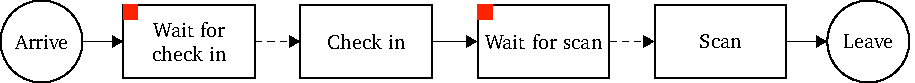
\includegraphics[width=155mm,height=\textheight]{chapters/clinic_1_cm/figures/patient_activity.pdf}

}

\caption{\label{fig-pat_act}Patient Activity Diagram}

\end{figure}%

\begin{figure}[htbp]

\centering{

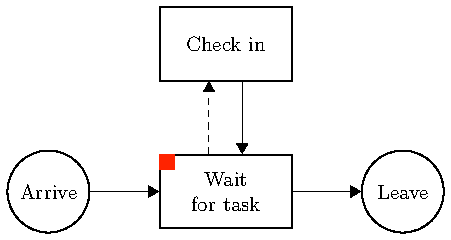
\includegraphics[width=76mm,height=\textheight]{chapters/clinic_1_cm/figures/receptionist_activity.pdf}

}

\caption{\label{fig-recep_act}Receptionist Activity Diagram}

\end{figure}%

\begin{figure}[htbp]

\centering{

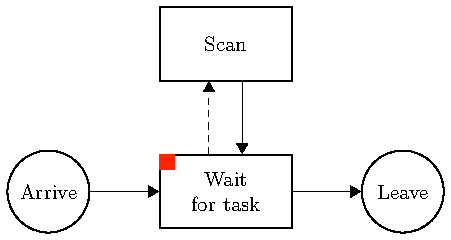
\includegraphics[width=76mm,height=\textheight]{chapters/clinic_1_cm/figures/CT_activity.pdf}

}

\caption{\label{fig-ct_act}CT Activity Diagram}

\end{figure}%

\newpage{}

\section{Logic}\label{logic}

\begin{table*}

\caption{\label{tbl-start_wait_check_in}OnStartWaitForCheckIn}

\centering{

\begin{tabular}{@{}>{\raggedright\arraybackslash}p{0.25cm}>{\raggedright\arraybackslash}p{13cm}@{}}
  \toprule
   & Triggered by: Patient p\\ \midrule 
  &
\begin{lstlisting}[language=CMPseudo]
receps = {r FOR r IN R IF r.State = "Wait for task (R)"}
IF receps IS NOT empty THEN 
    r_hat = argmin{r.CurrentStart FOR r IN receps}
    START Check In WITH p, r_hat
END IF
\end{lstlisting}
  \\ \bottomrule
  \end{tabular}

}

\end{table*}%

\begin{table*}

\caption{\label{tbl-start_wait_check_in}OnStartWaitForScan}

\centering{

\begin{tabular}{@{}>{\raggedright\arraybackslash}p{0.25cm}>{\raggedright\arraybackslash}p{13cm}@{}}
  \toprule
   & Triggered by: Patient p\\ \midrule 
  &
\begin{lstlisting}[language=CMPseudo]
cts = {c FOR c IN C IF c.State = "Wait for task (C)"}
IF cts IS NOT empty THEN 
    c_hat = argmin{c.CurrentStart FOR c IN cts}
    START Scan WITH p, r_hat
END IF
  \end{lstlisting}
  \\ \bottomrule
  \end{tabular}

}

\end{table*}%

\begin{table*}

\caption{\label{tbl-start_wait_check_in}OnStartWaitForTaskR}

\centering{

\begin{tabular}{@{}>{\raggedright\arraybackslash}p{0.25cm}>{\raggedright\arraybackslash}p{13cm}@{}}
  \toprule
   & Triggered by: Receptionist r\\ \midrule 
  &
\begin{lstlisting}[language=CMPseudo]
patients = {p FOR p IN P IF p.State = "Wait for Check In"}
IF patients IS NOT empty THEN 
    p_hat = argmin{p.CurrentStart FOR p IN patients}
    START Check In WITH p, r_hat
END IF
  \end{lstlisting}  
  \\ \bottomrule
  \end{tabular}

}

\end{table*}%

\begin{table*}

\caption{\label{tbl-start_wait_check_in}OnStartWaitForTaskCT}

\centering{

\begin{tabular}{@{}>{\raggedright\arraybackslash}p{0.25cm}>{\raggedright\arraybackslash}p{13cm}@{}}
  \toprule
   & Triggered by: CTMachine c\\ \midrule 
  &
\begin{lstlisting}[language=CMPseudo]
patients = {p FOR p IN P IF p.State = "Wait for Scan"}
IF patients IS NOT empty THEN 
    p_hat = argmin{p.CurrentStart FOR p IN patients}
    START Scan WITH p, r_hat
END IF
  \end{lstlisting}
  \\ \bottomrule
  \end{tabular}

}

\end{table*}%




\end{document}
